\chapter{Gestione delle reti}
Una rete di comunicazione viene concepita, implementata e gestita con uno o più \textit{scopi} come, ad esempio, una \textit{rete telefonica}, per comunicazioni vocali tra individui, una rete \textit{internet}, per il trasferimento e la condivisione di dati eterogenei, etc. Vi è molta differenza tra gli \textit{obiettivi} con cui una rete viene concepita (protocolli, standard, etc.) e quelli con cui questa viene \textit{gestita} dagli operatori; sicuramente il \textit{tempo} ed il \textit{business} sono due fattori determinanti.\\
Con il termine \textbf{management} si intendono tutte le operazioni che assicurano l'effettivo ed efficiente utilizzo di un sistema di comunicazioni e delle sue risorse in accordo con gli obiettivi aziendali. Si noti comunque che questa definizione è generica, può essere applicata anche a sistemi diversi da quelli di telecomunicazioni e gli \textit{obiettivi aziendali} possono essere correlati o meno con le telecomunicazioni.
\begin{figure}[htbp]
	\centering
	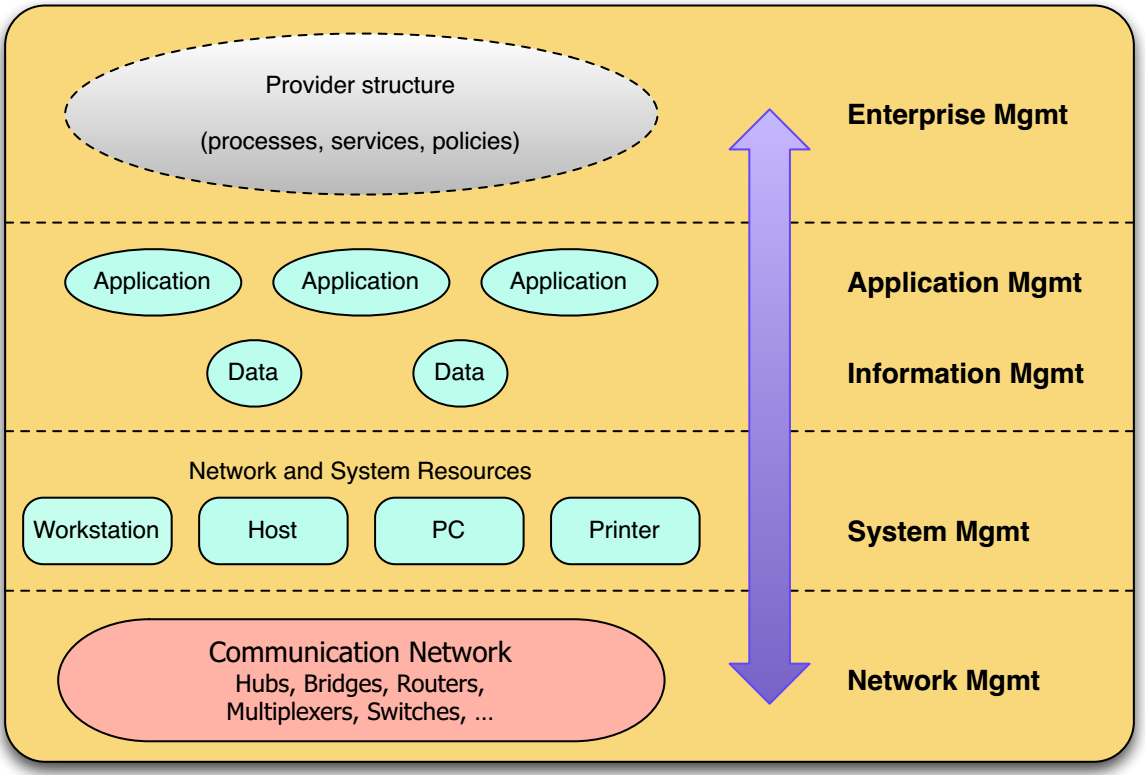
\includegraphics[scale = 0.4]{images/management_levels}
	\caption{Livelli di management.}
	\label{img:management_levels}
\end{figure}\\
In Figura \ref*{img:management_levels} sono rappresentati i livelli del management, iniziamo a descriverli dal basso. Il \textit{network management} mira ad occuparsi della gestione delle risorse di comunicazione, come ad esempio switch, router, linee, protocolli, etc., e dei servizi da essi offerti. Il \textit{system management} si occupa della gestione delle risorse dei sistemi finali e dei sistemi connessi alla rete (terminali, telefoni, servers, etc.). L'\textit{application management} tende ad occuparsi della gestione delle applicazioni distribuite (o meno) e dei servizi offerti in modo distribuito come e-mail e file sharing clusterizzato. Nell'\textit{enterprise management} o \textit{management integrato}, infine, tutti i livelli di management concorrono allo stesso scopo.
\begin{figure}[htbp]
	\centering
	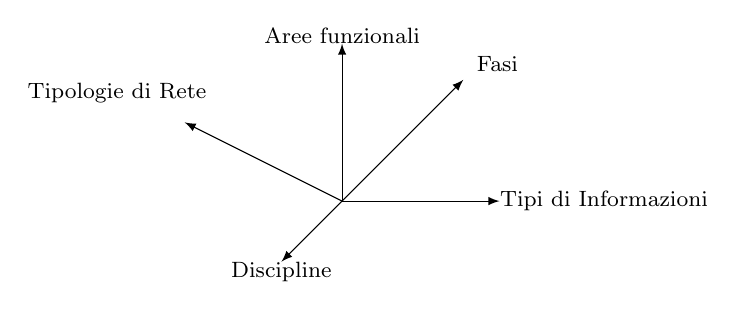
\begin{tikzpicture}
		\tikzset{mynode/.style={font=\footnotesize,inner sep=0pt,text=black}}
		%Begin plot
		\draw[-latex] (0,0,0) -- (2,0,0)node[mynode,anchor=west]{Tipi di Informazioni};
		\draw[-latex] (0,0,0) -- (0,2,0)node[mynode,anchor=south]{Aree funzionali};
		\draw[-latex] (0,0,0) -- (0,0,2)node[mynode,anchor=north]{Discipline};
		\draw[-latex] (0,0,0) -- (-2,1,0)node[mynode,anchor=north west,xshift=-2cm,yshift=0.5cm]{Tipologie di Rete};
		\draw[-latex] (0,0,0) -- (0,0,-4)node[mynode,anchor=north east,xshift=0.7cm,yshift=0.3cm]{Fasi};	
	\end{tikzpicture}
	\caption{Tipi di management.}
	\label{img:management_types}
\end{figure}\\
Come è possibile osservare dalla Figura \ref{img:management_types} vi sono vari tipi di management. Le \textit{aree funzionali} comprendono tutto ciò che riguarda configuration, performance, fault, security, accounting. Le \textit{fasi}, invece, planning, installation, operation, change, dismissing. Le \textit{tipologie di rete} comprendono internet, VPN, corporate, WAN, LAN, etc. Non esiste dunque un solo sistema di management e quindi non esiste una sola soluzione per il management, contando il fatto che non abbiamo parlato di organizzazione, fattori economici e legali, etc. Sostanzialmente l'idea fondamentale è quella di \textit{utilizzare concetti e formati standard per permettere l'interscambio di informazioni tra i fari livelli di management e tra le entità che lo compongono} (integrated management).

\noindent Vediamo adesso la \textit{management architecture}, ossia l'insieme degli standard relativi al management. Questa è suddivisa in:
\begin{itemize}
	\item \textbf{Information model}. Descrive il sistema sintattico e semantico per la rappresentazione delle risorse e delle informazioni in maniera orientata al management e indipendente dal venditore.
	\item \textbf{Communication model}. Descrive il sistema di accesso agli oggetti gestiti ed i protocolli di management.
	\item \textbf{Function model}. Organizza il sistema di management in sotto-task più gestibili e definisce funzioni di management generiche.
	\item \textbf{Organization model}. Definisce ruoli, modelli di cooperazione e domini di competenza.
\end{itemize}
L'unione dell'information e del communication model rappresenta gli \textquotedblleft elementi" hardware e software abbastanza comprensibili da un ingegnere, mentre l'unione di function ed organization model rappresenta gli \textquotedblleft elementi" organizzativi imprescindibili che coinvolgono persone e non macchine. Tutta questa architettura concorre a definire la \textbf{management platform}, che può (a volte) essere composta da elementi semplici, utilizzabili anche singolarmente (e.g. ping).

\noindent Per chi e perché viene attuato il management? In sostanza:
\begin{itemize}
	\item L'\textit{utente} finale è interessato ad avere un sistema affidabile, flessibile, sicuro, efficace, poco costoso, etc. e non è interessato a come viene realizzato. Tuttavia, le esigenze dell'utente sono alla base del management.
	\item L'\textit{azienda} vuole trarre profitti e anch'essa non è interessata a come un sistema viene realizzata. Tuttavia, anche le esigenze dell'azienda sono alla base del management.
\end{itemize}
Gli obiettivi del management devono dunque essere quelli di offrire all'utente il \textquotedblleft prodotto" (QoS, banda, whatever) richiesto e di gestire al meglio le risorse a disposizione evitando gli sprechi.

Una \textit{rete di telecomunicazioni} è progettata per offrire un servizio di comunicazione a distanza secondo modalità definite in un \textit{rapporto contrattuale}; quest'ultimo rappresenta la base del management. I soggetti coinvolti in questo rapporto sono sostanzialmente tre:
\begin{itemize}
	\item \textbf{Network operator}, cioè il gestore di rete. Si occupa di predisporre e di mantenere operativa l'infrastruttura necessaria al funzionamento dei servizi di telecomunicazioni utilizzando un supporto tecnico ed organizzativo. È sostanzialmente vincolato al rispetto dei requisiti di qualità per ognuno dei servizi supportati e di un costo di fornitura commisurato al beneficio ottenibile.
	\item \textbf{Service provider}, ossia il fornitore del servizio. Il service provider rende disponibili i servizi e le relative logiche di esecuzione che il cliente può personalizzare con modalità definite nei suoi impegni contrattuali (ivi compresi gli aspetti di qualità e costo). Utilizza inoltre le risorse dell'infrastruttura rese disponibili dal gestore di rete per trasferire l'informazione tra l'origine e la destinazione della comunicazione.
	\item \textbf{Service customer}, cioè il cliente che usufruisce del servizio.
\end{itemize}
Un \textit{servizio di telecomunicazione} è un servizio complesso che comprende: \textit{dispositivi terminali} (Terminal Equipment, TE) attraverso i quali l'utente usufruisce di uno o più servizi di telecomunicazione; \textit{dispositivi di accesso alla rete}; una \textit{rete} come piattaforma di connessione. Esso offre:
\begin{itemize}
	\item \textbf{Servizi applicativi}. Questi rispondono alle esigenze di comunicazione (in senso lato) degli utenti e comprendono, cioè, accanto alle problematiche connesse al trasferimento dell'informazione, anche aspetti legati all'utilizzazione finale.
	\item \textbf{Servizi di rete}. Rendono possibile il trasferimento dell'informazione tra due punti di accesso alla rete.
\end{itemize}
Generalmente abbiamo più \textit{tipologie di reti} di telecomunicazione, che si possono classificare in base a: \textit{profilo di utenza, mobilità dei terminali, estensione fisica, gamma dei servizi supportati}. La classificazione della rete aiuta a capire che tipo di management è necessario, quali tecnologie usare e, nel caso della sicurezza, è indispensabile per definire il \textit{Threat Model} visto in precedenza.

Per quanto riguarda le reti distinte in base al profilo di utenza abbiamo \textit{reti pubbliche} e \textit{reti private}. Nelle prime l'accesso è consentito a chiunque, previa stipulazione di un accordo contrattuale con il fornitore di servizi (e.g. Public Switched Telephone Network, PSTN). Nelle seconde gli utenti costituiscono un insieme chiuso ed omogeneo per quanto riguarda le esigenze di comunicazione e l'abilitazione all'accesso richiede la sottoscrizione di un accordo tra cliente e fornitore non assimilabile a quello definito in ambito pubblico (e.g. TErrestrial Trunked RAdio, TETRA).

Nelle reti distinte in base alla mobilità dei terminali, invece, abbiamo \textit{reti fisse}, \textit{reti mobili} e \textit{reti nomadiche}. Nelle prime i servizi supportati dalla rete sono accessibili solo da parte di utenti che non variano la propria posizione durante la comunicazione, oppure restano in un intorno limitato del punto di accesso alla rete; nelle seconde l'accesso è consentito ad utenti che non hanno alcun vincolo alla loro possibilità di movimento; nelle ultime, l'accesso è consentito ad utenti che non hanno alcun vincolo alla loro possibilità di movimento, ma durante la fruizione del servizio restano relativamente statici.

Per le reti distinte in base alla loro estensione abbiamo la \textit{rete in area locale} (Local Area Network, LAN), nelle quali l'area di interesse è limitata ad un singolo edificio o ad un complesso di insediamenti entro il raggio di qualche chilometro, la \textit{rete in area metropolitana} (Metropolitan Area Network, MAN) che fornisce servizi agli utenti che risiedono in una città o in una provincia, e le \textit{reti in area geografica} nelle quali gli utenti sono distribuiti su un'area molto estesa (una nazione, un continente, l'intero globo terrestre). Si noti che comunque questa classificazione non è più molto utile perché le tecnologie sono simili.

Infine, per reti distinte in base alla gamma dei servizi supportati abbiamo le \textit{reti dedicate ad un servizio} e le \textit{reti integrate nei servizi}. Le prime furono originariamente progettate e realizzate per offrire una sola tipologia di servizio (e.g. rete telegrafica/telefonica, rete per dati) e possono essere estese anche ad un insieme ristretto di altri servizi, pur con limitazioni severe per ciò che concerne la qualità conseguibile. Le seconde, invece, rendono possibile la fruizione di una vasta gamma di servizi di telecomunicazione con prestazioni di qualità e di costo superiori a quelli delle reti monoservizio.

La rappresentazione più intuitiva di una rete di telecomunicazione è data dal suo modello geometrico, ovvero dalla propria \textit{topologia}, nel quale gli elementi costitutivi sono i \textit{rami} e i \textit{nodi}. Un \textit{ramo} costituisce l'elemento di connessione di due nodi ed è rappresentato graficamente da un segmento \textit{orientato}, mentre un \textit{nodo} individua un elemento della rete connotato da specifiche funzionalità. Il significato di queste entità geometriche è diverso a seconda del tipo di operatività che si considera. Per gestire una rete è indispensabile conoscere la topologia della rete al giusto livello; si noti che non stiamo parlando di topologie a bus, anello, stella o altro.\\
Una rete esplica la funzione di trasferimento dell'informazione verso nodi preposti alla funzione di utilizzazione dell'informazione. In una rete si distinguono due sottoinsiemi di risorse funzionali dedicate al trasporto: \textit{rete logica} (svolge compiti di natura logica) e \textit{rete fisica} (svolge compiti di natura esclusivamente fisica). Le reti fisica e logica sono in stretta relazione gerarchica dato poiché le funzioni di natura logica utilizzano come supporto quelle fisiche e le funzioni di natura fisica sono al servizio delle altre. L'interazione tra rete fisica e rete logica segue il modello di interazione Client/Server in cui la rete logica agisce come Client e quella fisica come Server.\\
Una \textbf{rete logica} è un'infrastruttura che consente il trasferimento di informazioni da uno (o più) mittenti ad uno (o più) destinatari tra loro remoti e raggruppa funzioni di natura logica che hanno come obiettivo la la fornitura di un servizio di rete; nella formazione di un percorso logico nella rete sono coinvolti rami e nodi. Un \textit{ramo} individua un percorso diretto che l'informazione segue per essere trasferita da un punto all'altro e descrive gli apparati di rete che svolgono la funzione di multiplazione. Un \textit{nodo} individua il mezzo di scambio tra due o più rami che afferiscono ed è situato in corrispondenza degli apparati di rete che svolgono la funzione di commutazione. Ad esempio, se \textquotedblleft guardiamo" una rete a livello di indirizzi IP stiamo individuando una topologia logica che, tuttavia, potrebbe essere diversa a livello applicativo.\\
Una \textbf{rete fisica} è un'infrastruttura preposta al trasferimento dei segnali fisici che veicolano l'informazione. Sostanzialmente è la sede delle funzionalità di natura trasmissiva che coinvolgono tutti gli aspetti di propagazione del segnale ed è l'infrastruttura base a cui fa riferimento la rete logica. In questo caso, un \textit{ramo} individua il percorso fisico su cui avviene il trasferimento dei segnali e modella gli apparati trasmissivi presenti su quella tratta; un \textit{nodo} invece individua il punto di trasmissione e/o ricezione dei segnali ed è situato in corrispondenza dei terminali di ricetrasmissione. Dunque per \textit{rete fisica} si intendono ad esempio cavi, connettori, hub, switch etc. In generale le topologie della rete logica e della rete fisica non coincidono.

La rete si divide in più \textit{sezioni}: sezione di \textbf{accesso} (rete di accesso) e sezione \textbf{dorsale o interna} (rete di trasporto). La \textit{rete di accesso} consente agli utenti l'accesso alla rete con linea di utente individuale, può essere realizzata con svariati supporti fisici ed è la sede di di risorse indivise o, in altri casi, condivise; il punto di accesso alla rete comprende l'interfaccia utente-rete. La \textit{rete di trasporto} consente il trasferimento di informazione tra i nodi di accesso utilizzando eventualmente dei nodi di transito ed è la sede di risorse di trasferimento e di elaborazione condivise; ha come supporto una rete fisica generalmente a fibre ottiche. Nella pratica con il termine rete di accesso si indica la parte di rete destinata al collegamento fra la sede dei singoli utenti finali fino alla prima centrale di commutazione e più in generale al collegamento tra un utente e il suo provider; la rete di trasporto è la rete che distribuisce il traffico verso i vari provider.

\noindent Le informazioni che vengono scambiate all'interno di una rete sono di tre tipi:
\begin{itemize}
	\item \textit{Informazione di utente}. È il traffico che l'utente invia e riceve e per il quale è disposto a pagare (da qui il termine \textit{payload}, il traffico \textquotedblleft pagante"). Alcuni esempi: voce, suoni musicali, immagini, testi. L'informazione veicolata dalle reti di telecomunicazioni è sempre soggetta ad  un'operazione di \textit{codifica di sorgente/canale} che ne riduce la ridondanza e ne aumenta l'affidabilità in dipendenza dal mezzo trasmissivo. L'informazione di utente comprende anche l'informazione generata da una sorgente in relazione ad una specifica applicazione ed è destinata a uno o più collettori di informazione; può essere \textit{monomediale} (interessa un solo mezzo di rappresentazione) o \textit{multimediale} (coinvolge una pluralità di mezzi di rappresentazione). Genericamente è soggetta a QoS, ma la QoS richiesta è strettamente dipendente dal tipo di informazione e dall'utilizzatore (Human-Human, Human-Machine, Machine-Machine). L'informazione utente può anche essere soggetta a elaborazioni \textit{trasparenti} o \textit{apparenti} nel corso del trasporto.
	
	\item \textit{Informazione di segnalazione}. Costituisce quella parte di informazione che serve alla rete per funzionare in presenza di traffico di utente: è un traffico accessorio a quello utente che serve per far fluire l'informazione da una parte all'altra della rete in modo corretto (e.g. nel telefono: comporre un numero, individuare l'utente, inviare il numero del chiamante, etc.). Più precisamente possiamo dire che l'informazione di segnalazione (o di controllo) svolge una funzione di supporto per il corretto trasferimento dell'informazione di utente. Questo tipo di informazione è assente in caso di mancanza del traffico di utente. A livello pratico consente un'interazione tra cliente/utente e fornitore per:
		\begin{itemize}
			\item iniziare una comunicazione,
			\item negoziarne le caratteristiche qualitative e quantitative iniziali,
			\item modificare tali caratteristiche nel corso della comunicazione,
			\item aumentare le potenzialità dei servizi di base coinvolgendo le risorse di elaborazione che si rendono disponibili durante la comunicazione.
		\end{itemize}
	
	\item \textit{Informazione di gestione}. Costituisce il traffico che la rete produce per il suo normale e corretto funzionamento. Garantisce, cioè, il corretto svolgimento delle operazioni necessarie alla gestione delle risorse di rete relative all'erogazione dei servizi, al mantenimento del servizio, all'addebito del servizio. È necessario uno scambio di informazione di gestione tra le apparecchiature di rete e quelle terminali per un utilizzo efficiente dell'infrastruttura di rete. Esempi sono le tabelle di routing nel TCP/IP ed i keep-alive.
\end{itemize}
È importante ricordare che lo scopo di una rete è quello di trasportare la sola informazione dell'utente, tutto il resto (traffico di segnalazione e di gestione) costituisce \textit{overhead} ed occorre minimizzarlo.\\
Il trasferimento delle informazioni di utente, di segnalazione e di gestione può essere attuato sia nell'ambito di un'unica infrastruttura (come si preferiva in passato per le reti dedicate a un servizio) sia utilizzando infrastrutture separate in accordo alle impostazioni più moderne di integrazione dei servizi e di distribuzione dell'intelligenza all'interno della rete. In alcune reti, come SS7, informazioni di segnalazione e di gestioni sono logicamente separate dai dati; nei casi a canale comune è possibile sfruttare al meglio la banda totale del sistema, nei casi a canale separato si ha un maggior controllo del sistema poiché il canale di segnalazione e gestione non viene congestionato dalla trasmissione dati. A seconda del tipo di servizio che si vuole utilizzare funzionerà meglio uno o l'altro tipo. Si noti comunque che nel TCP/IP e nella rete Internet si usa un sistema di segnalazione e gestione a canale comune; nel caso di reti \textit{datagram oriented} l'informazione di segnalazione fa parte dell'header dei pacchetti (e.g. header IP).
\begin{figure}[htbp]
	\centering
	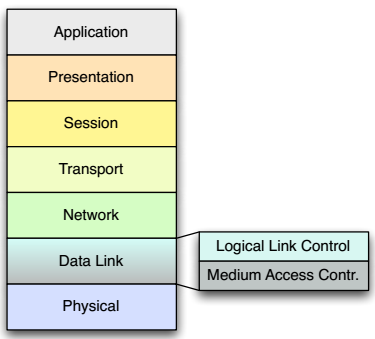
\includegraphics[scale = 0.55]{images/ISO-OSI}
	\caption{Modello ISO/OSI.}
	\label{img:ISO-OSI}
\end{figure}\\
In Figura \ref{img:ISO-OSI} è rappresentato il modello ISO/OSI. È importante sapere due concetti riguardanti questo modello: \textit{information hiding} (non esporre l'implementazione, ma solo un servizio) e \textit{separation of concerns} (non duplicare le funzionalità). La maggior parte dei problemi odierni del TCP/IP deriva dalla violazione di questi due concetti. Un problema fondamentale del modello ISO/OSI è dovuto al fatto che il traffico utente, di segnalazione e di controllo non possono separati e non vi è possibilità di fare il \textit{cross layer}, ovvero saltare da un layer all'altro. Un esempio di pila protocollare che permette di ovviare a questi problemi è una pila tridimensionale (e.g. ATM): a fianco dei layers dati vi è un unico layer di segnalazione, dietro ai quali vi è un unico layer di controllo.\\
Le reti wireless e wired che prenderemo in considerazione nel seguito sono 802.3 (ethernet), 802.11 (WiFi), 802.1 e LTE.
\begin{figure}[htbp]
	\centering
	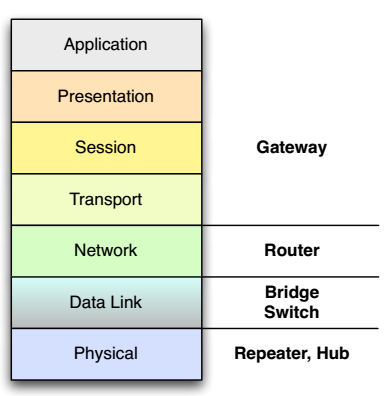
\includegraphics[scale = 0.55]{images/network-devices}
	\caption{Dispositivi di rete.}
	\label{img:network-devices}
\end{figure}\\
I dispositivi che operano nelle reti ed in Internet (Figura \ref{img:network-devices}) sono differenziati in base al livello protocollare in cui operano. A livello fisico abbiamo \textit{repeater} (due porte) e \textit{hub} (più porte). A livello collegamento abbiamo i \textit{bridge} (connettono tecnologie diverse ma compatibili usando il Logical Link Control e cambiando un frame da un tipo ad un altro purché compatibili -- e.g. frame 802.11 in frame ethernet) e gli \textit{switch} (connette tecnologie uguali, instradando i pacchetti verso l'indirizzo desiderato). A livello rete abbiamo i \textit{router}, dispositivi che lavorano a livello di indirizzi IP e che decidono l'instradamento basandosi su tabelle e protocolli di apprendimento delle route. Ai livelli superiori si parla di \textit{gateway}. Il fatto che questi dispositivi siano dotati di \textquotedblleft intelligenza" (i.e. managed) non significa che operino a livelli superiori a quello di riferimento (e.g. uno switch managed opera sempre a livello 2, anche se presenta un'interfaccia di gestione web). Dato che il TCP/IP occupa i livelli 3 e 4, in Internet vi sono solo routers e gateways.

\section{Internet}
Internet non è nata un giorno a caso: la sua nascita è stata il risultato di un processo lungo, lento e contrastato; se vogliamo capire cos'è e come sopravvive, è fondamentale capire come e perché si è venuta a creare. Le idee rivoluzionarie vennero agli inizi degli anni '60 soprattutto da due persone: Leonard Kleinrock e J.C.R. Licklider. Il primo introdusse le comunicazioni a pacchetto in un momento in cui era norma fare delle comunicazioni a messaggio (messaggi lunghi); il secondo, anche se meno famoso, diede dei contributi notevoli soprattutto nell'ambito delle comunicazioni spaziali. Internet \textquotedblleft nasce" quindi intorno agli anni '60 grazie alle idee di Kleinrock e Licklider, poi finanziate in modo massiccio dal Dipartimento della Difesa Americano (DoD); nasce dunque come rete finanziata dai militari, ma essendo un progetto di ricerca venne reso aperto. Il \textit{come} ed il \textit{perché} Internet abbia battuto la concorrenza di tutti i modelli di rete presenti al tempo, è un problema complesso che coinvolge \textit{fattori economici}, \textit{fattori tecnologici}, \textit{facilità di utilizzo}, \textit{utilizzatori finali} e \textit{politica}.

\noindent Nella storia di Internet troviamo i pattern fondamentali di una rete di telecomunicazioni:
\begin{enumerate}
	\item \textit{Target} (user-driven o provider-driven). Normalmente quando si crea una rete vi sono uno o più soggetti che effettuano la standardizzazione, un provider che costruisce la rete e degli utenti che la utilizzano; deve esserci inoltre un \textit{business model} che prevede un \textit{investimento} ed un \textit{ritorno di investimento} dopo $x$ anni. In Internet questo modello si ribalta perché nasce da un progetto di ricerca (che serve alla ricerca), e non è mirato ad un ritorno di investimento.
	\item \textit{Finanziamento dello startup}. Successivamente Internet prese piede ed il Dipartimento della Difesa Americano decise di tagliare i fondi poiché gli Internet Service Provider erano in grado di essere autonomi.
	\item \textit{Riposizionamento del target}. Internet nacque puramente come una rete dati e nel corso degli anni si è evoluta per avere protocolli più sicuri ed esigenti, per supportare le esigenze degli utenti.
	\item \textit{Concorrenza da parte di altri}. Vi è stata ed è tuttora presente una concorrenza a livello protocollare, di proposte (e.g. la \textquotedblleft guerra dei browser", modifiche proposte all'HTTP, ...); più precisamente vi è una concorrenza riguardante i modelli di rete ed i modelli di business.
	\item \textit{Evoluzione tecnologia dei servizi}.
\end{enumerate}
Fino alla fine degli anni '70 Internet vide un'evoluzione tecnologica \textquotedblleft di base" ed una concorrenza da parte delle reti a \textit{modello verticale}. Una rete a modello verticale è una rete studiata per trasportare uno o più servizi, la cui evoluzione è conseguente ai servizi stessi; nella pratica si hanno dispositivi ed un'infrastruttura che funzionano solo se prodotti dalla stessa azienda, quindi solo se hanno un preciso modello proprietario. In una rete verticale non vi è una separazione netta tra il fornitore dei servizi e quello del trasporto. Internet è un \textit{modello orizzontale}: si fornisce una serie di protocolli che (by design) sono progettati per essere pronti all'utilizzo o, alternativamente, per essere estesi utilizzando protocolli già esistenti o creandone dei nuovi. Negli anni '80-'90 vi fu l'apertura dei mass-market (passaggio da rete di ricerca a rete commerciale), lo sviluppo dei servizi, la concorrenza sui servizi e, conseguentemente, sulla rete stessa. Allo stato attuale vi sono dei segnali di ritorno a reti verticali, che potrebbero causare la fine della rete aperta.

Internet è uno dei rarissimi esempi di rete nella quale vi è una separazione quasi perfetta tra fornitori di servizi e quelli del trasporto; questo è dovuto alla sua origine \textquotedblleft accademica" ed al fatto che non sia nata per vendere un servizio. Le caratteristiche principali di Internet sono le seguenti:
\begin{itemize}
	\item È basata sui protocolli TCP/IP,
	\item Comprende anche molti altri protocolli (UDP, ICMP, ARP, RIP, OSPF, protocolli di livello applicativo...), e formati (RFC 822, MIME...),
	\item È una rete di \textquotedblleft sotto-reti" che collega più di $110\,000$ sotto-reti con più di 50 milioni di calcolatori,
	\item È standardizzata con RFC (Request For Comment),
	\item I collegamenti fisici tra host e router sono basati su: LAN, MAN, canali punto-punto in fibra od in cavo coassiale, reti X.25, ISDN, ponti radio, Frame Relay, ATM, SLIP, PPP, il tutto in un sistema aperto,
	\item Esistono realizzazioni TCP/IP anche per reti non standard.
\end{itemize}
\begin{figure}[htbp]
	\centering
	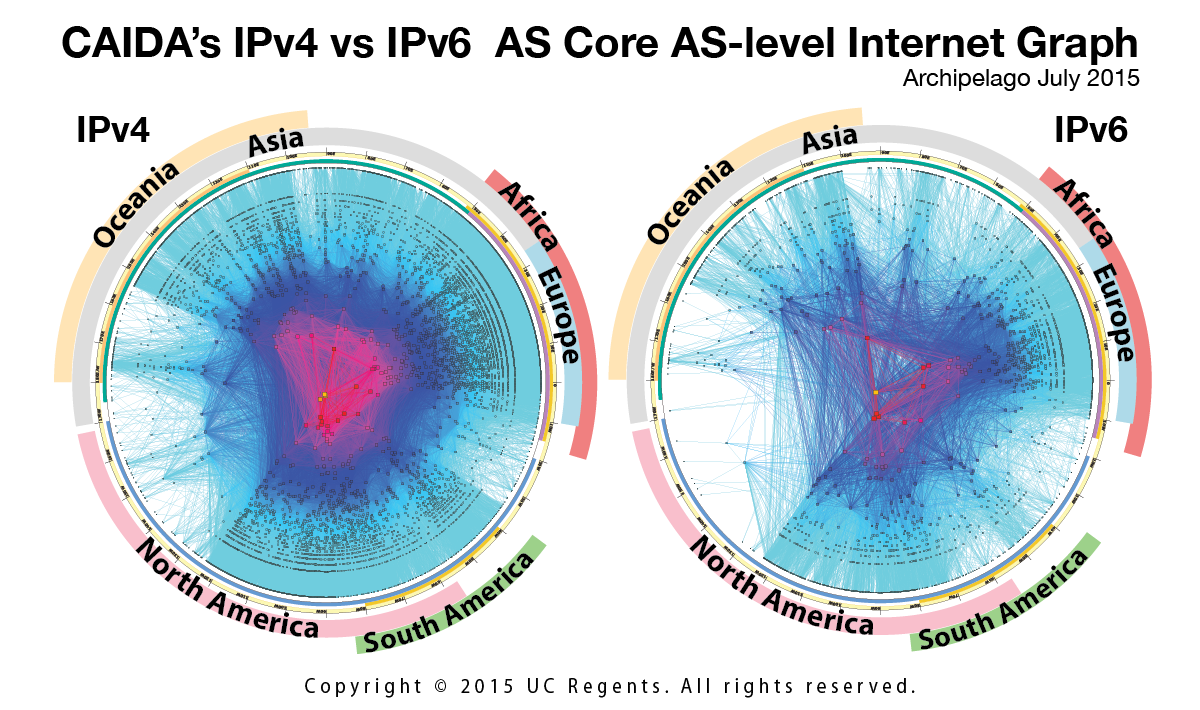
\includegraphics[scale = 0.3]{images/ascore-2015}
	\caption{Topologia della rete Internet riguardante la distribuzione di link tra Autonomous System (AS) (2015).}
	\label{img:ascore-2015}
\end{figure}
In Figura \ref{img:ascore-2015} è rappresentata la distribuzione mondiale dei link tra AS (un blocco di indirizzi IP, un ISP, ...), riguardante sia IPv4 sia IPv6; attualmente la crescita di IPv6 dipende quasi interamente dagli Internet Service Provider. Quando le due mappe saranno pressoché uguali, IPv6 sarà ad un buon livello della propria diffusione e sarà possibile iniziare ad eliminare IPv4.\\
Fissiamo la terminologia che useremo d'ora in avanti: \textit{subnet} e \textit{Autonomous System} (AS). Una \textit{subnet} è un segmento di rete basata su TCP/IP delimitato dai suoi confini di routing. È identificabile a livello rete da una coppia Indirizzo/Subnet Mask, oppure da un indirizzo espresso secondo notazione CIDR (in IPv6 dai primi 64 bit dell'indirizzo). Si noti che (in IPv4) una subnet finisce con un router: due subnets non possono comunicare se non attraverso un router. Il concetto di \textit{Autonomous System} (AS) è di tipo amministrativo e si riflette solo sul routing: \textquotedblleft\textit{Within the Internet, an autonomous system (AS) is a collection of connected Internet Protocol (IP) routing prefixes under the control of one or more network operators that presents a common, clearly defined routing policy to the Internet (cf. RFC 1930, Section 3)}". In generale all'interno di un AS sono definiti dei protocolli di routing che possono essere diversi da quelli utilizzati all'esterno per connettere più AS; questo perché un amministratore di un AS può decidere in modo arbitrario cosa fare e quali servizi fornire all'interno del proprio AS.\\
Per quanto riguarda la struttura di Internet, possiamo dire che questa è una inter-rete che consente a sistemi terminali (host) appartenenti a sotto-reti eterogenee di scambiare informazioni. Non possiede un organismo centralizzato dotato di poteri di controllo e lo sviluppo tecnologico si basa sul contributo degli utenti della rete stessa. È basata sulla pila protocollare TCP/IP e l'interconnessione tra sotto-reti è un paradigma fondamentale; non è prevista tuttavia la traduzione dei protocolli. Si noti che vi è una separazione amministrativa e di management tra le diverse sotto-reti che, nel modello, non sono tenute ad una gestione integrata. Per \textquotedblleft sotto-reti" non si intendono le \textquotedblleft subnets", bensì gli \textit{Autonomous System} (AS).\\
La pila protocollare TCP/IP è situata a livello rete (e superiori): i protocolli TCP/IP assumono che le sotto-reti non eseguano nessuna funzione a parte quella di trasferimento delle unita informative ed esiste la possibilità di duplicazione delle funzioni tra strati TCP/IP e strati protocollari specifici di una sotto-rete. Le entità di Internet sono gli \textit{host} ed i \textit{router/gateway}: gli \textit{host} (L7) sono le sorgenti e le destinazioni delle informazioni univocamente riconosciuti nella rete (tramite indirizzo IP); i \textit{router/gateway} (L3/L4-7) sono i nodi intermedi che instradano i pacchetti IP tra le sotto-reti e possiedono un'interfaccia per ogni sotto-rete a cui sono connessi.\\
Vediamo brevemente il \textit{principio di interconnessione}. L'host sorgente, dopo aver fatto una traduzione dell'indirizzo alfanumerico in un indirizzo IP:
\begin{enumerate}
	\item Forma il pacchetto IP diretto all'host di destinazione (si ha un indirizzo di livello 3).
	\item Determina se l'host di destinazione si trova sulla sua stessa subnet: se la subnet è la stessa, viene determinato l'indirizzo MAC dell'host di destinazione; se la subnet è diversa, viene determinato l'indirizzo IP e l'indirizzo MAC del router verso cui inviare il pacchetto. In base alle informazioni di livello 3 viene deciso il tipo di routing (diretto o indiretto).
	\item Consegna il pacchetto alla rete che lo rimanda al destinatario (router o host). L'indirizzo di livello 3 viene tradotto in un indirizzo di livello 2 (MAC).
\end{enumerate}
In sostanza un router elabora l'indirizzo dei pacchetti IP e determina, tramite la propria tabella di routing, la subnet in cui si trova l'host di destinazione: se l'host di destinazione si trova in una delle subnets a cui il router è direttamente connesso, affida il pacchetto alla subnet per la consegna, altrimenti determina il router successivo verso il quale instradare il pacchetto. Una subnet, invece, si occupa di trasferire i pacchetti IP incapsulandoli nelle proprie unità dati ed utilizzando i protocolli propri.\\
In Internet esistono tre livelli di identificazione di un indirizzo:
\begin{itemize}
	\item \textbf{Indirizzo MAC}. È l'indirizzo della scheda di rete e solitamente è prefissato.
	\item \textbf{Indirizzo numerico}. È l'indirizzo IP (e.g. 150.217.8.24) ed è assegnato dal gestore della rete in base al tipo di rete a cui si appartiene (subnet).
	\item \textbf{Indirizzo alfanumerico}, ad esempio \texttt{lenst.det.unifi.it}. È un indirizzo libero ed è sufficiente che sia mappato in un NameServer.
\end{itemize}
\begin{figure}[htbp]
	\centering
	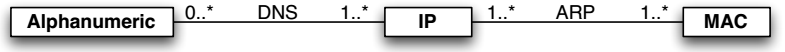
\includegraphics[scale = 0.5]{images/UML-address}
	\caption{Diagramma UML degli indirizzi in Internet.}
	\label{img:UML-address}
\end{figure}
In Figura \ref{img:UML-address} è riportato un banale diagramma UML che mette in relazione i tre tipi di indirizzi. L'indirizzo IP è l'unico indirizzo assegnato in modo pseudo-geografico perché, dal momento che l'indirizzo IP è necessario per il routing, vi è la necessità di avere in qualche modo un'associazione tra indirizzi e località spaziali. In particolare, un indirizzo IP:
\begin{itemize}
	\item Identifica un host; se un host è connesso a più di una rete (multi-homed) avrà un indirizzo IP per ogni rete.
	\item È unico un tutta la rete ed ha una lunghezza di 32 bit.
	\item È assegnato ad una macchina su base geografica, ovvero in base alla rete a cui è connessa.
	\item In origine, nel 1981, era formato da due parti: \textit{net\_id} (identificativo della subnet) e \textit{host\_id} (identificativo dell'host all'interno della subnet). Quindi \textit{IP\_Address} $=$ \textit{net\_id}.\textit{host\_id}.
\end{itemize}
Originariamente la divisione tra \textit{net\_id} e \textit{host\_id} non era fissa, ma dipendeva dalla \textit{classe} dell'indirizzo. La struttura di indirizzamento a due livelli gerarchici era sufficiente nella fase iniziale di Internet. Nel 1984 e stato aggiunto un terzo livello gerarchico: il livello di Sottorete (Subnet), in cui si utilizzano alcuni bit della parte di \textit{host\_id} per codificare il \textit{subnet\_id}.
\begin{figure}[htbp]
	\centering
	\begin{bytefield}{32}
		\bitheader{0,7,8,15,16,23,24,31}\\
		\begin{rightwordgroup}{Classe A}
			\bitbox{1}{0} & \bitbox{7}{Net ID} & \bitbox{24}{Subnet ID + Host ID}
		\end{rightwordgroup} \\
	\end{bytefield}
	\begin{bytefield}{32}
		\begin{rightwordgroup}{Classe B}
			\bitbox{2}{10} & \bitbox{14}{Net ID} & \bitbox{16}{Subnet ID + Host ID}
		\end{rightwordgroup} \\
	\end{bytefield}
	\begin{bytefield}{32}
		\begin{rightwordgroup}{Classe C}
			\bitbox{3}{110} & \bitbox{21}{NetID} & \bitbox{8}{S ID + H ID}
		\end{rightwordgroup} \\
	\end{bytefield}
	\caption{Classi di indirizzi IP.}
	\label{img:address-classes}
\end{figure}\\
In Figura \ref{img:address-classes} sono riportate le tre classi di indirizzi IP. Si noti che il routing avviene sulla NetID. Questo metodo di routing che prevedeva l'utilizzo delle tre classi di indirizzi IP era comodo originariamente, ma si è dimostrato inefficiente in seguito, poiché, così facendo, un router dovrebbe avere una tabella di routing di dimensioni $2^7-2+2^{14}-2+2^{21}-2 = 2\,113\,658$. Venne quindi introdotta la notazione \textbf{CIDR} (\textbf{C}lassless \textbf{I}nter\textbf{D}omain \textbf{R}outing), nella quale gli indirizzi sono nella forma \texttt{x.x.x.x/y} (e.g. 150.217.8.0/24) dove \texttt{y} indica il numero di bit della NetID (contando da sinistra). All'interno dei router il CIDR viene utilizzato in un modo lievemente diverso, ovvero per accorpare linee e ridurre la dimensione della tabella di routing; ad esempio due indirizzi che differiscono di un solo bit vengono \textquotedblleft accorpati" in: 150.217.8.0/24 $+$ 150.217.9.0/24 $=$ 150.217.8.0/23.
\begin{table}[htbp]
	\centering
	\begin{tabular}{|l|l|l|l|l|l|l|l|}
		\hline
		\textbf{Destination} & \textbf{Gateway} & \textbf{Genmask} & \textbf{Flags} & \textbf{Metric} & \textbf{Ref} & \textbf{Use} & \textbf{Iface} \\ \hline
		10.8.0.2 & * & 255.255.255.255 & UH & 0 & 0 & 0 & tun0 \\ \hline
		10.4.0.1 & * & 255.255.255.255 & UH & 0 & 0 & 0 & tun1 \\ \hline
		192.168.21.0 & 10.8.0.2 & 255.255.255.0 & UG & 0 & 0 & 0 & tun0 \\ \hline
		150.217.8.0 & * & 255.255.255.0 & U & 0 & 0 & 0 & eth0 \\ \hline
		192.168.2.0 & 10.4.0.1 & 255.255.255.0 & UG & 1 & 0 & 0 & tun1 \\ \hline
		10.8.0.0 & 10.8.0.2 & 255.255.255.0 & UG & 0 & 0 & 0 & tun0 \\ \hline
		192.168.11.0 & * & 255.255.255.0 & U & 0 & 0 & 0 & eth2 \\ \hline
		default & detfw.det.unifi & 0.0.0.0 & UG & 0 & 0 & 0 & eth0 \\ \hline
	\end{tabular}
	\caption{Esempio di tabella di routing.}
	\label{tab:routing-table-example}
\end{table}
Nella Tabella \ref{tab:routing-table-example} è riportato un esempio reale di tabella di routing; abbiamo una destinazione, un gateway (cioè il next-hop), la genmask (i.e. netmask), dei flag, una metrica (definisce, in caso di due linee totalmente equivalenti quale delle due scegliere), ref e use (servono per vedere quante volte è stata utilizzata la linea e se questa è aggiornata o se è da rimuovere), I(nter)face (indica l'interfaccia utilizzare per inoltrare i pacchetti). Se due destinazioni presentano lo stesso gateway (e la stessa interfaccia), possono essere accorpate modificando la genmask. Per identificare la destinazione di un pacchetto occorre scoprire la entry a massima verosimiglianza. In particolare, indicando con $\&\&$ l'AND logico bit a bit, se
$$\text{DestIP}\;\&\&\;\text{RTMask}_i == \text{RTDestIP}_i$$
(RT = Routing Table) allora la entry $i$ ha rank pari al numero di bit a uno della RTMask e si sceglie la entry a rank maggiore, ossia scegliamo la entry che ha più bit ad uno della RTMask; nel caso in cui si ottenga più di un risultato, si confrontano le metriche.

\section{Routing}
Abbiamo visto che il \textit{routing} potrebbe essere un problema di non poco conto. Fondamentalmente esistono due tipi di routing: \textit{diretto} ed \textit{indiretto}. Nel routing diretto si utilizzano i meccanismi della subnet alla quale si è associato, ossia ARP (per IPv4) e NDP (per IPv6). Nel routing indiretto, invece, il router cerca una entry nella routing table. Ciò che ci interessa vedere è, dunque, come viene costruita una routing table (RT) in un router. Prima di andare avanti, però, dobbiamo ricordare alcuni punti.\\
\begin{itemize}
	\item Il routing è composto da due elementi: un \textit{protocollo di routing} per costruire le RTs, che viene eseguito periodicamente a prescindere dai pacchetti dati, ed un \textit{algoritmo di switching}, che si applica ad ogni pacchetto in transito.
	\item In genere le RTs non vengono mai costruite a mano, tranne in casi particolari.
	\item Le RTs non possono cambiare troppo spesso perché, altrimenti, non funzionerebbero più i protocolli di Congestion Control del TCP; inoltre è da tenere presente che gli algoritmi di routing sono limitati dalla velocità della rete di segnalazione.
	\item Il routing non viene fatto \textquotedblleft a caso": deve avere un \textit{obiettivo}, un funzionale da minimizzare.
	\item Il routing influenza il funzionamento della rete; è compito del management guidare il routing, e non essere guidati da esso.
\end{itemize}
Abbiamo visto che esiste il routing diretto ed indiretto, ma esiste un'ulteriore classificazione: il \textit{routing IGP} (Interior Gateway Protocol), che avviene all'interno di un AS, ed il \textit{routing EGP} (Exterior Gateway Protocol), che avviene tra AS differenti. Si noti che questi non sono protocolli, ma \textit{classi di protocolli}; vediamoli nel dettaglio.

Dal momento che un AS è un dominio amministrativo unico, si suppone che il gestore di rete possa (e debba) individuare un criterio ottimale all'interno dell'AS, in modo da ottimizzare i percorsi. Lo scopo dei protocolli \textit{IGP} è quello di applicare il criterio ottimale individuato dal gestore e di creare automaticamente le tabelle di routing che minimizzino il funzionale di costo scelto: è sostanzialmente un problema di ricerca del minimo. Da un punto di vista teorico è una questione semplice, dobbiamo: definire un funzionale di costo $f:\mathbb{R}^n\to\mathbb{R}$ (preferibilmente semplice e convesso), associare un costo ad ogni ramo (e/o nodo, ad esempio nel caso in cui si voglia minimizzare l'energia utilizzata da un nodo), ed applicare un algoritmo di ricerca del minimo per ogni coppia $(i,j)$ di nodi. È banale dimostrare che è sufficiente associare il costo ai rami, ma il problema è come realizzare l'idea.\\
Una qualsiasi rete a pacchetto può essere modellata come un \textit{grafo orientato e pesato} in cui i nodi sono i router ed i rami sono le linee trasmissive o intere subnets: questa è la topologia logica della rete a livello IP. L'instradamento (routing) di un pacchetto equivale alla ricerca di un cammino (minimo) nel grafo associato della rete. Per ogni nodo sorgente esisterà un albero che lo connette a tutti i possibili nodi destinazione (non tutta Internet, stiamo parlando a livello di AS). Dunque in un AS con $N$ nodi di hanno $N^2$ alberi. Un router non deve tuttavia conoscere tutti gli alberi, è sufficiente che conosca il next-hop relativo a tutte le possibili destinazioni all'interno dell'AS; per avere questa conoscenza non è necessario calcolare gli $N^2$ alberi.\\
Per quanto riguarda il costo dei rami è possibile utilizzare due strategie: \textit{costo fisso} e \textit{costo dinamico}. La prima strategia può essere considerata se il costo di un ramo è legato alla sua esistenza: assegniamo $costo = 1$ se il ramo esiste, $costo = \infty$ altrimenti. Questo algoritmo non genera un overhead considerevole, ma genera alberi molto statici e funziona bene sono se il carico su un ramo (o la congestione di nodo) non sono fattori importanti. Sostanzialmente il costo fisso viene usato per reti che hanno cambiamenti nel tempo molto lenti. La seconda strategia è decisamente più complessa della prima: è necessario decidere un funzionale di costo e può generare soluzioni instabili per le quali occorre fare attenzione. Il costo dinamico viene usato per reti che hanno cambiamenti nel tempo molto frequenti. In entrambi i casi il routing è \textit{dinamico}, perché è generato automaticamente.\\
Un classico esempio di algoritmo di routing a costo fisso è il \textbf{RIP} (RIP v2: RFC 2453). Il costo di un ramo, detto \textit{metric}, è fisso e tale che $metric \in [1, \dots, 15]$; il valore $metric = 16$ indica un link down. L'algoritmo implementato è di tipo \textit{distance vector} (non ha bisogno di memorizzare la topologia della rete), nel quale si minimizza una \textquotedblleft distanza" generalizzata rappresentata dal parametro \textit{metric}. In pratica ogni nodo scambia con i vicini diretti (i router è cui e connesso direttamente, i next-hop) un pacchetto RIP; il router ricevente analizza il pacchetto e, se indica un percorso con metrica inferiore a quella già contenuta nella sua RT, aggiorna la RT. Il limite a 16 di \textit{metric} è imposto per ovviare al problema del link down. In pratica, se un link non è più disponibile, a questo viene associato un costo infinito ed un nodo adiacente non lo può raggiungere. Il nodo adiacente chiede dunque agli altri suoi vicini se possiedono una rotta per il nodo non raggiungibile e questi, non essendo stati ancora aggiornati del link down, rispondono erroneamente indicando un certo numero di hop. Si innesca così un meccanismo ciclico per cui inizia ad aumentare sempre più il numero di hop per raggiungere il nodo \textquotedblleft irraggiungibile" (questo problema prende il nome di \textit{counting-to-infinity}); per limitare questa crescita infinita, il primo router che raggiunge $metric = 16$ pone fine al ciclo ed aggiorna i vicini. Più è alto il massimo valore di \textit{metric}, più la rete impiega ad \textquotedblleft accorgersi" di un link down. Il RIP ha, dall'altro lato, un limite intrinseco per i 16 \textquotedblleft hop", che limita pesantemente le possibilità di differenziare i link su reti \textquotedblleft larghe" (i link dovrebbero quindi essere più o meno tutti uguali). È semplice riconoscere che questo è un algoritmo Bellman-Ford: alla ricezione di un pacchetto questo viene confrontato con le entry nella RT e se necessario viene aggiornata la RT. Se indichiamo con $|V|$ il numero di vertici e con $|E|$ il numero di archi del grafo, questo algoritmo necessita di $O(|V|\cdot|E|)$ passi per essere eseguito. Ogni passo è tuttavia eseguito ogni 30 secondi a causa del timer di invio dei pacchetti RIP, dunque se ad esempio prendessimo $|V|=40$ e $|E|=50$, l'algoritmo impiegherebbe oltre 16 ore per essere eseguito. Inoltre la convergenza lenta non permette, ad esempio, di legare la metrica alla congestione dei rami. In realtà non è esattamente così: esiste un algoritmo di routing, detto \textit{triggered-updates} per cui, quando cambia una tabella di routing, il messaggio di update dei vicini viene inviato dopo circa due secondi; questo permette dei tempi di convergenza ragionevoli. Vi sono varie versioni del RIP: il \textit{RIPv1}, in cui l'autenticazione ed il CIDR sono assenti (da non usare), il \textit{RIPv2} nel quale sono presenti l'autenticazione ed il CIDR, è retro-compatibile con RIPv1 e gestisce la differenza tra routes interior e exterior (dell'AS), ed \textit{RIPng}, che è identico al RIPv2, ma progettato per IPv6.\\
Un esempio di algoritmo di routing a costo dinamico è l'\textbf{OSPF (Open Shortest Path First)}. Attualmente OSPFv2, descritto nell'RFC 2328, è per IPv4, mentre OSPFv3, descritto nell'RFC 2740, è per IPv6: vi sono poche differenze effettivamente, l'obiettivo è quello di unirli in un unico protocollo. In questo tipo di algoritmo si ha che il costo di un ramo (\textit{metric}) è dinamico, il parametro \textit{metric} è abbastanza grande da non creare problemi ed implementa un Link State Routing (ha bisogno di memorizzare la topologia della rete). Lo standard dell'OSPF ordina inoltre di utilizzare l'algoritmo di Dijkstra: se indichiamo con $|V|$ il numero di vertici e con $|E|$ il numero di archi del grafo, questo algoritmo necessita di $O(|E|+|V|\log |V|)$ passi per essere eseguito. Computazionalmente parlando è ancora piuttosto complesso: una volta ricevuti i dati (LSA), il router deve calcolare la propria tabella di routing prima dell'arrivo dei dati successivi. Ogni router ha quindi un limite massimo di numero di vertici e di archi che può supportare. Dal momento che il costo è associato ed ogni router, per decidere la RT, deve conoscere tutti i costi dei rami, è indispensabile che un router conosca l'intera topologia della rete (nel RIP non è necessario). In particolare, i router hanno la responsabilità di contattare i router adiacenti (cioè tutti i router che condividono con esso una parte della rete) e di acquisire la loro identità con dei pacchetti di Hello. I router formano quindi dei Link State Advertisement (LSA), contenenti una lista delle reti adiacenti con i relativi costi di raggiungimento, che verranno poi trasmessi a tutti gli altri router. Dunque tutti i router della rete avranno lo stesso insieme di dati e quindi potranno costruire lo stesso grafo pesato della rete, utilizzato per determinare i cammini ottimi e quindi l'instradamento. In questo processo vi è sia un grande carico computazionale sia un grande overhead. Dunque abbiamo che per il RIP la complessità computazionale influisce sulla velocità di convergenza, mentre nell'OSPF la complessità computazionale è un limite che influisce sulla potenza di calcolo della CPU del router. Per limitare i problemi di complessità computazionale e di carico di rete, OSPF viene organizzato in modo \textit{gerarchico} (in aree) all'interno di un AS (Figura \ref{img:OSPF}).
\begin{figure}[htbp]
	\centering
	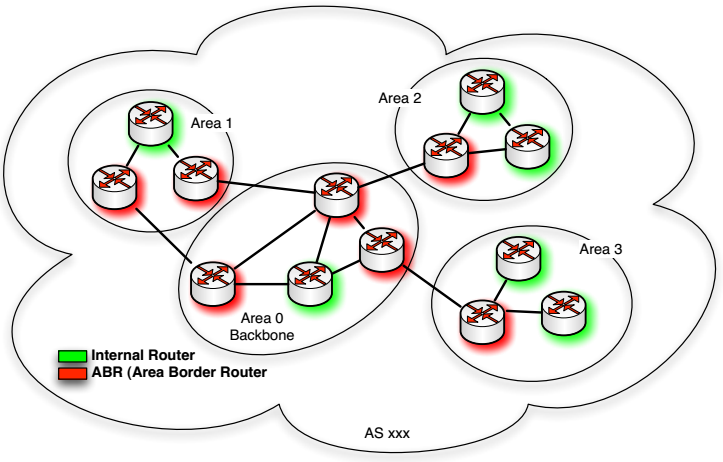
\includegraphics[scale = 0.5]{images/OSPF}
	\caption{Organizzazione gerarchica di OSPF.}
	\label{img:OSPF}
\end{figure}\\
In particolare esiste un'area speciale detta \textit{area di backbone} che connette tutte le altre aree (numerate); la definizione delle aree è lasciata al network manager. Gli unici requisiti da rispettare sono due: tutti i router di ogni area devono essere interconnessi e le varie aree devono essere connesse solo tramite backbone. All'interno di ciascuna area l'algoritmo di routing è OSPF che calcola il path minimo tra i router di quell'area. Il risultato di utilizzare OSPF in un AS è quello di \textit{non} ottenere il percorso migliore (globale), perché questo non è la \textquotedblleft somma" di tutti i percorsi ottimi all'interno di un'area (locali).\\
Vediamo quindi brevemente l'\textit{inizializzazione} di OSPF:
\begin{enumerate}
	\item Si effettua una inizializzazione e controllo (attraverso i livelli inferiori) delle interfacce.
	\item Si inviano degli \textit{Hello} in broadcast per acquisire le informazioni sui router vicini.
	\item Si ricevono gli \textit{Hello} dei vicini, che vengono anche utilizzati per testare il funzionamento dei link (keep alive).
\end{enumerate}
Nelle aree multi-accesso si elegge un \textit{designated router}, mentre l'altro router è di backup. Così facendo si limitano sia il traffico sia la complessità del grafo di rete. Periodicamente si inviano \textit{LSA (Link State Advertisement)} per fornire informazioni topologiche e per notificare cambiamenti nello stato dei router e dei links. A regime viene costruito il database topologico della rete (dai LSA), ciascun router calcola lo shortest-path tree a lui relativo e lo shortest-path tree genera la tabella di routing. Vi sono cinque tipi di pacchetto OSPF:
\begin{itemize}
	\item \textbf{Hello}. Stabilisce e mantiene le relazioni con i vicini.
	\item \textbf{Database description}. Descrive il contenuto del database topologico. Questi messaggi sono in genere scambiati quando viene inizializzata un'adiacenza.
	\item \textbf{Link-state request}. Richiede parti del database topologico dai router vicini. Questo tipo di messaggio viene scambiato dopo che un router scopre (esaminando i pacchetti di descrizione del database) che parti del proprio database topologico sono obsolete.
	\item \textbf{Link-state update}. Risponde ad un pacchetti di tipo link-state request. Questi messaggi sono utilizzati anche per la dispersione regolare di LSAs. In un singolo pacchetto di tipo link-state update può essere incluso più di un LSA.
	\item \textbf{Link-state acknowledgment}. Accetta i pacchetti di tipo link-state update.
\end{itemize}
Un concetto da precisare ulteriormente per quanto riguarda OSPF è l'\textit{adiacenza}: due router si considerano adiacenti se appartengono alla stessa area. Quindi, il traffico di OSPF è grande (per una rete grossa ho sia problemi di capacità computazionale sia dei problemi di overhead, perché i LSAs devono essere mandati da un nodo a tutti i nodi appartenenti alla stessa area) e tutti i router di una stessa area hanno lo stesso database topologico. I LSAs vengono inviati a tutti i router adiacenti, tramite flooding o multicast.
\begin{figure}[htbp]
	\centering
	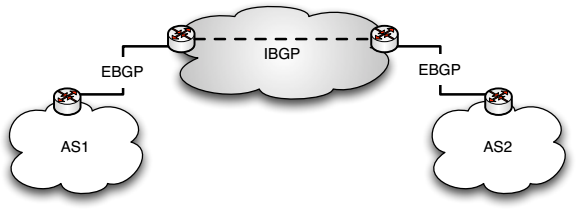
\includegraphics[scale = 0.5]{images/BGP}
	\caption{IBGP e EBGP.}
	\label{img:BGP}
\end{figure}\\
Vediamo adesso i protocolli di routing \textit{EGP}. Tra AS diversi \textit{non} è possibile utilizzare protocolli di routing IGP; il motivo principale è la mancanza di una funzione da minimizzare. Dal momento che gli AS sono domini amministrativi diversi, è impensabile poter \textquotedblleft ottimizzare" una funzione, perché il costo dei link è dipendente da fattori non quantificabili su una scala condivisa. I protocolli EGP tendono dunque a minimizzare altro, come parametri locali e fattori commerciali. Il protocollo EGP più diffuso è il \textit{BGP} (Border Gateway Protocol) e ne esistono due varianti (Figura \ref{img:BGP}):
\begin{itemize}
	\item \textbf{IBGP} (Interior BGP). Viene utilizzato all'interno di un AS e serve per far comunicare (a livello logico) i suoi router di bordo. Le rotte interne all'AS sono sempre e comunque determinate da un IGP.
	\item \textbf{EBGP} (Exterior BGP). Viene utilizzato tra due diversi AS. Normalmente opera su un link punto-punto.
\end{itemize}
\begin{figure}[htbp]
	\centering
	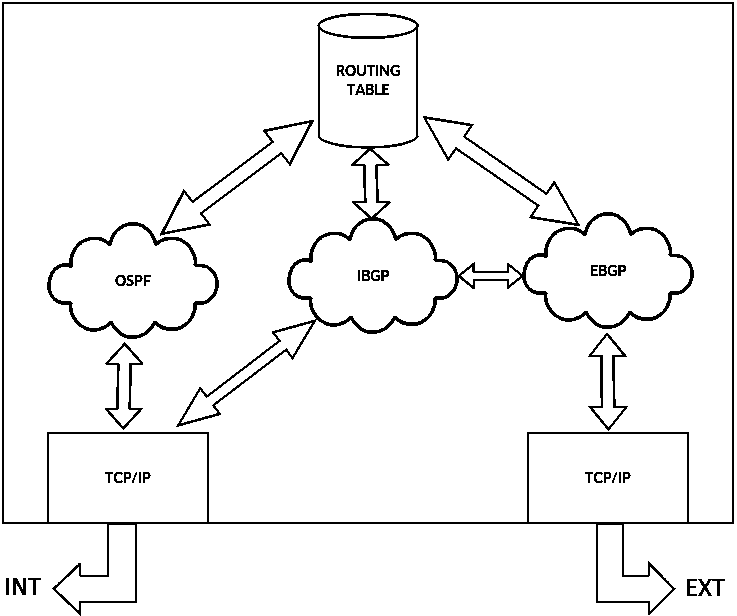
\includegraphics[scale = 0.35]{images/BGP-internal}
	\caption{Struttura interna di un router di bordo.}
	\label{img:BGP-internal}
\end{figure}
In Figura \ref{img:BGP-internal} è rappresentata la struttura logica interna di un router di bordo, ovvero di un router che risiede al confine di un AS e si occupa di collegare fra loro più AS. Questo avrà un'interfaccia verso l'esterno ed una o più interfacce verso l'interno. Sull'esterno vi è il protocollo EBGP, sull'interno vi è l'IBGP ed un protocollo interno (e.g. OSPF). Questi tre protocolli convivono tramite la RT. Quando arriva la dichiarazione di una rotta raggiungibile dall'esterno (exterior) tramite EBGP, questa viene scritta nella RT come rotta esterna e viene propagata, con eventuali parametri, tramite IBGP in tutto l'AS; si noti che i parametri possono essere specificati da IBGP e non da OSPF. I parametri non sono quelli standard di un protocollo di routing interior, ma dei parametri locali (interni ai router):
\begin{itemize}
	\item \textbf{Weight}. È un attributo locale non propagato (advertised). In caso di multipath, viene preferita la route con weight più grande.
		\begin{figure}[htbp]
			\centering
			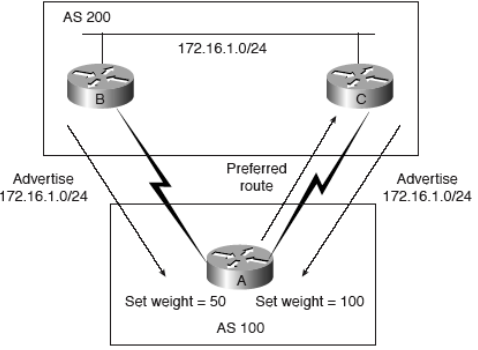
\includegraphics[scale = 0.4]{images/weight}
			\caption{Weight.}
			\label{img:weight}
		\end{figure}
	Con riferimento alla Figura \ref{img:weight}, supponiamo di avere un AS di destinazione (AS 100) ed un AS di partenza (AS 200). Entrambi i link vengono realizzati con Advertisement di una data subnet. La rotta da preferire è quella a weight maggiore. Il weight può essere ad esempio riferito al tipo di collegamento (e.g. wireless o fibra).
	\item \textbf{Local preference}. Si hanno due router di ridondanza in entrambi gli AS (Figura \ref{img:local-preference}).
		\begin{figure}[htbp]
			\centering
			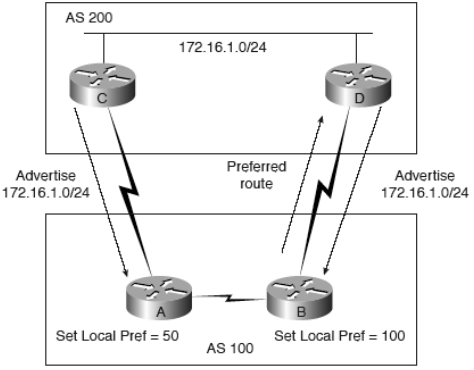
\includegraphics[scale = 0.4]{images/local-preference}
			\caption{Local preference.}
			\label{img:local-preference}
		\end{figure}
	È usato per scegliere la strada di \textit{uscita} preferita tra due o più router. In caso di multi-route viene preferita la route con maggior peso. Tra i due router dell'AS 100 vi è una comunicazione IBGP per mettersi d'accordo su quale dei due utilizzare, in base al local preference, per andare in quella sottorete. Una volta decisa, l'informazione tornerà ai router dell'AS 200 che avranno come \textit{preferred route} D-B. C toglierà dalla propria routing table usata da OSPF il link verso A.
	\item \textbf{Multi-exit discriminator (MED) o metric attribute}. È utilizzato per suggerire la strada di \textit{ingresso} preferita tra due o più router. In caso di multi-route, viene preferita la route con minor peso.
		\begin{figure}[htbp]
			\centering
			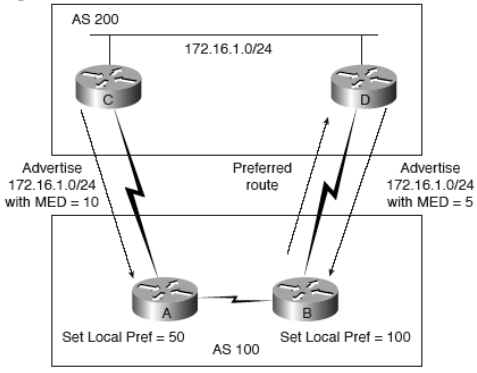
\includegraphics[scale = 0.4]{images/MED}
			\caption{Multi-Exit Discriminator Attribute.}
			\label{img:med}
		\end{figure}
	Sostanzialmente è il caso contrario di quello precedente. Se il local preference rappresenta una decisione del local AS, il MED rappresenta una dichiarazione di preferenza dell'altro AS.
	\item \textbf{Origin}. È utilizzato per classificare il modo con cui BGP ha appreso una route. In particolare, le route sono divise in:
	\begin{itemize}
		\item \textbf{IGP}. La route è generata da un protocollo IGP ed è interna all'AS che la propaga.
		\item \textbf{EGP}. La route è stata appresa attraverso un protocollo EGP.
		\item \textbf{Incomplete}. La route è di origine sconosciuta o appresa tramite altra via (e.g. inserita a mano).
	\end{itemize}
	Questa classificazione è utilizzata per la scelta della tabella di routing: in genere si preferiscono secondo l'ordine IGP, EGP, Incomplete. Questo perché, se ad esempio si fosse data priorità maggiore ad un EGP piuttosto che ad un IGP, potrebbe essere selezionata una rotta esterna per arrivare ad un router del proprio AS.
	\item \textbf{AS\_path}. È utilizzato per determinare i loop: ogni router di un AS traversato viene aggiunto ad una lista ordinata e vengono scartate tutte le routes che contengano loops (individuando se nel path vi è due volte lo stesso router).
	\item \textbf{Next hop}. È utilizzato per indicare il next-hop (indirizzo IP del router che fa l'advertising). Nell'EBGP è l'indirizzo IP dell'advertiser, mentre nell'IBGP il next-hop viene lasciato inalterato: è quindi necessario avere un IGP all'interno dell'AS oppure utilizzare delle routes statiche all'interno dell'AS. La route viene altrimenti scartata.
	\item \textbf{Community}. È utilizzato per raggruppare destinazioni (comunità) per le quali le decisioni di routing debbano subire speciali trattamenti. Sostanzialmente serve per limitare la distribuzione di una rotta.
	\begin{figure}[htbp]
		\centering
		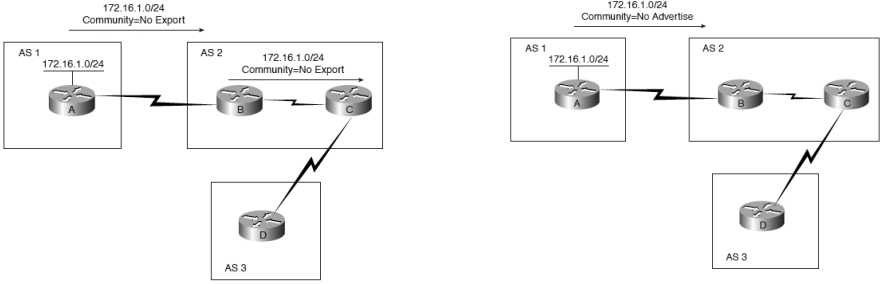
\includegraphics[scale = 0.5]{images/community}
		\caption{Community.}
		\label{img:community}
	\end{figure}
	Per definire le comunità si usano le \textit{route maps}. Le comunità preferite sono:
	\begin{itemize}
		\item \textbf{Internet}. Advertising libero senza alcuna restrizione.
		\item \textbf{No-Export}. Non esportare la route tramite EBGP: rimane all'interno dell'AS.
		\item \textbf{No-Advertise}. Non esportare la route a nessuno.
	\end{itemize}
	La community è stata ideata per questioni di sicurezza (non voglio che una rotta passi attraverso AS non fidati, che potrebbero usarla) e di accordi commerciali tra AS diversi (si decide se far passare o meno dati attraverso la propria infrastruttura di rete). Con riferimento alla Figura \ref{img:community}, è possibile vedere come nel primo caso il router dell'AS 1 trasmetta l'indirizzo della subnet, chiedendo esplicitamente di non ri-esportarlo all'esterno dell'AS 2; nel secondo caso, invece, l'indirizzo non viene esportato neppure ai router dell'AS 2. In entrambi i casi AS 3 non è a conoscenza del collegamento fra AS 1 e AS 2.
\end{itemize}
Per stabilire una route, i router BGP si scambiano quindi queste informazioni riguardanti la raggiungibilità di una rete e una serie di attributi relativi al link (o ai link) tra i due AS coinvolti. Come può essere già intuito, BGP non è un protocollo che ottimizza globalmente i percorsi: abbiamo solo una serie di minimi locali. I minimi locali vengono riconosciuti attraverso un funzionale non continuo. In particolare, quando si riceve un aggiornamento, si procede alla scelta del path secondo la seguente logica:
\begin{enumerate}
	\item Se il path specifica un next hop inaccessibile, scarta l'update.
	\item Scegli il path con maggior weight (locale).
	\item Se sono uguali, scegli il path con maggior local preference.
	\item Se sono uguali, scegli il path originato dal BGP che gira sul router stesso.
	\item Altrimenti, scegli il path con l'AS\_path più corto.
	\item Se sono uguali, scegli in base all'origin (IGP $>$ EGP $>$ incomplete)
	\item Altrimenti, scegli il path con il MED più basso.
	\item Altrimenti, scegli il path esterno piuttosto che quello interno.
	\item Altrimenti, scegli il path attraverso l'IGP più vicino.
	\item Altrimenti, scegli il path con il numero IP più basso, secondo quanto specificato dall'ID del router BGP.
\end{enumerate}
Si noti che non vi sono regole che fanno riferimento alla community, perché questa agisce già, a livello generale, sull'esportabilità della route; questa procedura viene fatta sui dati che si hanno, dunque la community ha già agito in precedenza. Inoltre, l'unico punto sul quale è possibile compiere dell'ottimizzazione è il quinto (sul numero di hop) e si può notare immediatamente che non è un'ottimizzazione globale. Infine, la regola dieci, che apparentemente è priva di senso, in realtà vuole rappresentare la regola di default, cioè la regola che si vuole attuare in caso di fallimento delle condizioni precedenti. Quello che si vuol fare nell'ultima regola è evitare la casualità imponendo una scelta (arbitraria, ma fissata) dalla quale è possibile capire che siamo finiti nel caso di default.

Dunque, non è prevista nessuna regola sulla minimizzazione della distanza né sulla banda tra AS diversi e non vi è ottimizzazione o minimizzazione end-to-end. La somma dei minimi locali \textit{non} garantisce la scelta di un path globale ottimo. Lo scopo del BGP è invece quello di avere dei \textit{percorsi stabili e raggiungibili}. Dal BGP dipendono quindi la connettività globale di Internet, la stabilità dei link e le priorità.

\section{Quality of Service}
La \textbf{Quality of Service (QoS)} si riferisce ai meccanismi di controllo delle risorse che influiscono sulla qualità di un servizio (sono quantità misurabili in modo oggettivo, e.g. banda). La QoS è la capacità di fornire diverse priorità a diverse applicazioni, utenti o flussi di dati, o per garantire un certo livello di prestazioni per un flusso di dati.\\
La \textbf{Quality of Experience (QoE)} è una misura soggettiva dell'esperienza di un utente con un venditore. La QoE dipende dalla QoS.\\
La base di tutto è la QoE, ovvero la soddisfazione dell'utente, che è dipendente dal \textit{servizio} e dalle \textit{aspettative} dell'utente. In una rete \textit{monoservizio} la QoE è un semplice problema relativo alla gestione della rete, mentre nelle reti \textit{multiservizio} la QoE dipende da come vengono gestiti nella rete i vari tipi di flussi dati. Alcuni pacchetti devono avere infatti una gestione diversa, altrimenti non è possibile avere un servizio adeguato.

La QoS deve essere effettuata a tutti i livelli di rete, con un approccio cross-layer. A livello applicazione vi è lo sviluppo di API capaci di riservare trattamento diverso ai servizi Real-time a livello di sistema operativo, a livello trasporto i protocolli devono essere differenziati per servizio (QoS end-to-end), a livello rete vi deve essere una differenziazione dei flussi a livello IP (QoS router-to router), a livello collegamento vi è una differenziazione dei flussi a livello di frame o celle (QoS sul link), ed a livello fisico devono essere presenti mezzi trasmissivi più efficienti (rame, fibra ottica), tecniche di codifica, BER adattiva.

Nel 2001 Sprint (un grande ISP americano) sosteneva che la QoS non serve, perché se si ha a disposizione una banda pressoché infinita non vi sono problemi di trasmissione. In realtà Sprint stava adottando una politica di \textit{over-provisioning}, per cui aveva un'infrastruttura di rete (anche con diverse fibre per lo stesso link) a capacità trasmissiva ed a banda molto elevata. Infatti, il costo maggiore per la realizzazione di un'infrastruttura di rete sono gli scavi per far passare i collegamenti, non la singola fibra in sé. Dunque, non appena il traffico raggiungeva un livello sufficientemente alto, semplicemente veniva allocata più banda. Ciò che serviva secondo Sprint era la Quality of Access (QoA); le reti di dorsale europee sono molto più congestionate e con capacità inferiori. Purtroppo l'over-provisioning non è così semplice in Europa.

In sostanza le tecniche di QoS servono a raggiungere il grado desiderato di QoE; tuttavia la QoE non è dipendente dalle tecniche che vengono usate (l'utente non ne è al corrente), quindi qualsiasi mezzo per ottenere la QoE è lecito. Esistono differenti metodi per ottenere la QoE.\\
Un esempio concreto di tipi diversi di traffico è il traffico di tipo \textit{non real-time} (TCP) ed il traffico \textit{real-time} (UDP). Il primo è di tipo Burst, richiede un tasso di errore praticamente nullo, tutti i pacchetti sono trattati allo stesso modo e potrebbero essere ricevuti con un certo ritardo. Il secondo è un flusso di tipo continuo, accetta un certo numero di errori, i pacchetti hanno priorità diverse e devono essere ricevuti con il minor ritardo possibile.\\
Un altro esempio è il VoIP. Se andiamo a misurare la qualità di una comunicazione VoIP, potremmo usare i seguenti parametri: tasso di perdita di pacchetti IP, delay e delay Jitter (variazione del delay). La QoS risultante è mostrata in Tabella \ref{tab:voip-table}.
\begin{table}[htbp]
	\centering
	\begin{tabular}{l|c|c|c|c}
		& Scarsa & Media & Buona & Ottima \\ \hline
		Packet Loss (\%) & 25 & 10 & 3 & 0 \\ 
		Delay (ms) & $>450$ & 450 & 250 & $<150$\\
		Jitter (ms) & 225 & 125 & 75 & 0
	\end{tabular}
	\caption{Tabella dei parametri di QoS VoIP.}
	\label{tab:voip-table}
\end{table}\\
Il delay Jitter è il parametro più difficile da rispettare. Se vogliamo una buona qualità dobbiamo quindi avere un ritardo basso e pochissimo accodamento nei buffer. La presenza di una coda implica infatti un Jitter; togliendo la coda e buttando quindi alcuni pacchetti, non abbiamo Jitter. Dunque la QoS è sostanzialmente un trade-off tra packet loss, delay e Jitter. Esiste un altro metodo per evitare il riempimento delle code: AQM (Active Queue Management).

Per diminuire il Jitter a destinazione vi è un \textit{buffer di playout}. Tutti i flussi RT (Real-Time) hanno caratteristiche di isocronicità (grossomodo), o quantomeno devono essere usati dal player allo stesso rate di emissione della sorgente. La trasmissione in rete introduce perdite e ritardi, ma soprattutto altera i riferimenti temporali intra-pacchetto (Jitter). Per recuperare la desincronizzazione si deve usare un buffer di playout che è dipendente dal Jitter, ma che però introduce un ulteriore ritardo. In sostanza: se è troppo piccolo si cominciano a perdere pacchetti e/o a non averne di disponibili; se è troppo grande si introduce troppo ritardo. Un esempio di buffer di playout è quello di YouTube, ossia la barra grigia che ne indica il riempimento.

La QoS end-to-end deve garantire livelli di servizio accettabili in \textit{tutti} gli elementi della catena di comunicazione. Sorgono problemi quando il link end-to-end attraversa reti di ISP diversi: servono accordi di \textit{peering} e di \textit{Service Level Agreement} fra gli ISP. Un problema risiede nel fatto che non tutte le reti sono uguali, ciascuna ha le proprie criticità: accesso (pochi utenti, banda limitata), core (molti utenti, banda molto elevata), tecnologie differenti. Non è sufficiente creare un backbone ad alta velocità per ridurre la dipendenza dalla QoS ed esistono reti in cui non è possibile fare affidamento sulla larga banda.

Per la QoS servono differenti strategie nelle diverse parti di rete. In particolare possiamo parlare di \textit{QoS nei nodi di rete} e \textit{QoS end-to-end}. La prima è sostanzialmente a livello IP: shaping del traffico, scheduling dei pacchetti, classificazione, riservazione delle risorse, etc. La seconda può coinvolgere anche i livelli protocollari superiori con meccanismi di segnalazione end-to-end, architetture di rete per la QoS, etc.\\
In un nodo si possono implementare diverse funzioni relative alla QoS, ma non tutte sono applicabili in tutti i punti della rete a causa del carico computazionale che richiedono. Queste sono:
\begin{itemize}
	\item \textbf{Classifier}. Osserva i pacchetti IP entranti nel nodo e li classifica in base al loro indirizzo IP, Port Number e al tipo di protocollo superiore.
	\item \textbf{Marker}. Provvede a \textquotedblleft marchiare" i pacchetti con una QoS a seconda di come sono stati classificati dal Classifier.
	\item \textbf{Traffic Policer}. Esegue un condizionamento del traffico, osservando il rate possibile ed agendo di conseguenza. In pratica confronta il traffico con le policy definite nel Service Level Agreement (contratto con ISP).
	\item \textbf{Traffic Shaper}. Modella il flusso sulla porta di uscita in modo da ottimizzare il throughput, sulla base delle istruzioni fornite Traffic Policer.
	\item \textbf{Scheduler}. Genera più code all'interno del nodo di rete e usa algoritmi di scheduling delle code, evitando o gestendo le congestioni di rete. È l'elemento che influenza di più la QoS.
\end{itemize}
\begin{figure}[htbp]
	\centering
	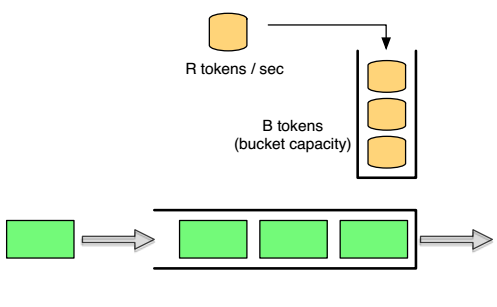
\includegraphics[scale = 0.5]{images/token-bucket}
	\caption{Token Bucket.}
	\label{img:token-bucket}
\end{figure}
Un esempio di algoritmo di Traffic Policy (o Shaper) nei nodi di rete è il Token Bucket (Figura \ref{img:token-bucket}). Quando un pacchetto arriva al router, viene tolto dal Bucket un certo numero di Tokens (dipendentemente dalla dimensione del pacchetto); un pacchetto non potrà essere inviato se non ci sono Tokens a sufficienza nel Bucket. Il router trasmetterà un burst di pacchetti minore o uguale a $B$, ad un rate minore o uguale ad $R$. Lo scopo principale è quello di limitare il rate medio di pacchetti.

Gli algoritmi di scheduling nei nodi di rete sono molto simili a quelli che si trovano nei Sistemi Operativi, hanno gli stessi obbiettivi e gli stessi difetti. Vediamo tre tipi di scheduler:
\begin{enumerate}
	\item \textbf{Scheduler ottimo}. Uno scheduler ottimo sarebbe quello che si avvicina al limite del \textit{Fluid Scheduling}, ossia ad uno scheduler che tende a dividere i dati in unità piccolissime. Sfortunatamente le \textquotedblleft unita" di scheduling sono i pacchetti, oltre non è possibile scendere.
	\item \textbf{Scheduler non Work Conserving}. È uno scheduler che può essere inattivo in qualche istante, ma può garantire alcune proprietà, come le deadlines. Se succede qualcosa di imprevisto, si è in grado di interrompere il task in corso.
	\item \textbf{Scheduler Work Conserving}. È uno scheduler che è inattivo solo quando non vi è più traffico da spedire. Non è possibile tuttavia interrompere un task in corso, ossia non è strettamente a priorità.
\end{enumerate}
Gli algoritmi di scheduling nei router sono uno dei punti più delicati.

A volte le code di ricezione si riempiono e buttare via i pacchetti quando la coda è piena (\textit{tail-drop}) è la cosa sbagliata. Il \textit{queue management} è strettamente legato al \textit{congestion control}, perché il TCP (e molti altri protocolli) rilevano le congestioni misurando il numero di pacchetti persi. Sostanzialmente servono ad evitare congestioni: si fornisce un feedback attivo al trasmettitore prima che la coda diventi piena. Un esempio di come questo viene fatto è l'algoritmo \textbf{WRED (Weighted Random Early Detection)}, di cui vediamo gli aspetti principali:
\begin{itemize}
	\item I pacchetti vengono scartati dal nodo di rete con probabilità tanto maggiore quanto più la coda è piena (RED).
	\item Si fissano dei limiti per la lunghezza della coda ed a seconda del loro superamento si scartano i nuovi pacchetti in arrivo.
	\item La probabilità di scarto può dipendere in modo pesato dal tipo di classe cui appartengono (WRED).
	\item Sfrutta rate adattivo del TCP, che vede lo scarto del pacchetto come dovuto a congestione, e dunque rallenta il rate in trasmissione; non funziona con UDP.
\end{itemize}
Si noti che quella appena descritta è una tecnica atta ad \textit{evitare} la congestione sul nodo di rete, anziché gestirla una volta avvenuta.

In Internet ci sono sostanzialmente due modelli di gestione della QoS: \textbf{Integrated Services (IntServ)} (Giugno 1994, RFC 1633) e \textbf{Differentiated Services (DiffServ)} (Dicembre 1998, RFC 2475). Non sono più utilizzati per problemi pratici.\\
Il modello IntServ prevede di \textit{prenotare le risorse} necessarie al mantenimento della QoS richiesta in \textit{ogni apparato} di rete attraversato da un flusso dati. Il flusso è inteso come sequenza di pacchetti con stesso indirizzo IP sorgente e destinazione e stessi Port numbers. Ogni router della rete deve allocare risorse (banda, memoria, etc.) a
sufficienza per ciascun flusso e ciascun router della rete deve avere un \textit{per-flow state} relativo a ciascun flusso a cui viene data QoS. Poiche le risorse su ogni router sono limitate, ciascun router dovrà controllare e decidere quali flussi allocare e quali rifiutare: per questo esiste un \textit{Admission Control}. Il modello IntServ ha tre componenti base:
\begin{itemize}
	\item \textbf{Traffic Classes}. Classi di servizio ottenibili da un flusso. I parametri di ciascuna classe possono essere modificati a piacimento.
	\item \textbf{Traffic Control}. Esegue controllo sul traffico che transita su ogni nodo di rete. È composto da vari sotto-componenti.
	\item \textbf{Setup Protocol}. Costituisce il sistema di segnalazione fra i nodi di rete per l'allocazione delle risorse. È anche la base per l'Admission Control.
\end{itemize}
Le Classi di Traffico (Traffic Classes) ammissibili sono tre:
\begin{enumerate}
	\item \textbf{Default}. È il servizio Best Effort dell'Internet attuale, anche se non è una vera Traffic Class.
	\item \textbf{Guaranteed Service}. Supporta traffico Real-Time che richiede un ritardo di propagazione limitato. Offre una \textit{garanzia} sulla QoS offerta.
	\item \textbf{Controlled Load Service}. Approssima un servizio di tipo Best Effort su una rete \textit{non congestionata} (avere prestazioni ottimali).
\end{enumerate}
La definizione del Guaranteed Service nasconde un grosso problema: la garanzia. Per ottenere davvero un Guaranteed Service si dovrebbe usare un non work conserving scheduler, dunque di solito si usa il Controlled Load Service. Il Traffic Control viene effettuato tramite tre sotto-sistemi:
\begin{enumerate}
	\item \textbf{Admission Control}. Controlla che le risorse sul router e nella rete possano supportare un particolare servizio richiesto.
	\item \textbf{Packet Classifier}. Esamina indirizzo IP e Port Number per vedere la classe a cui appartiene.
	\item \textbf{Packet Scheduler}. Effettua lo scheduling dei pacchetti per trasmetterli alla porta di uscita del router (usando ad esempio WFQ).
\end{enumerate}
Ovviamente nel caso di un router c'è anche una sezione relativa al forwarding dei pacchetti.
\begin{figure}[htbp]
	\centering
	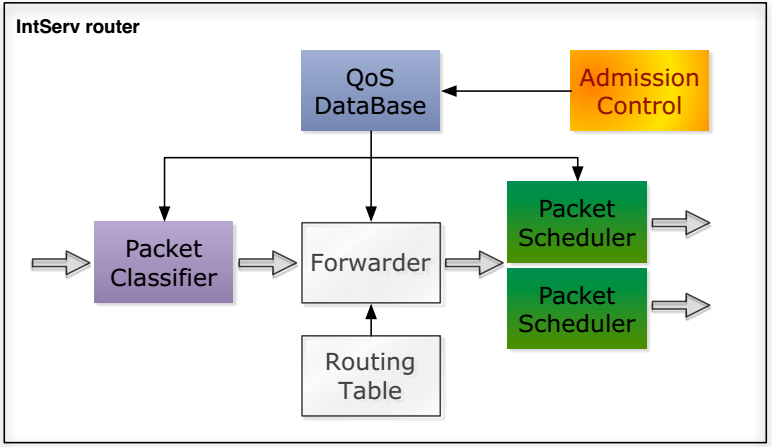
\includegraphics[scale = 0.4]{images/int-serv-router}
	\caption{Schema di un nodo IntServ.}
	\label{img:int-serv-router}
\end{figure}
In Figura \ref{img:int-serv-router} è rappresentato lo schema di ogni IntServ router. Vi è un classificatore di pacchetti per riconoscere se un pacchetto appartiene ad un flusso gestito e che deve essere confrontato con un database QoS; l'admission control viene utilizzato solo se il pacchetto appartiene ad un flusso nuovo. Vi è poi un forwarder che, sulla base della decisione presa e della routing table, decide di inoltrare il pacchetto, che andrà agli scheduler. Gli scheduler agiranno di conseguenza alla QoS decisa. Un limite di IntServ risiede routing table, che è diversa da quella normalmente usata: se è stato allocato un path per far comunicare due host, questo potrebbe cambiare nel corso della trasmissione per vari motivi (e.g. decisi dall'IGP), e la routing table deve essere \textquotedblleft interrotta" (per flussi con QoS). Inoltre, se vi è un guasto, il flusso va negoziato, ed Packet Classifier può rivelarsi computazionalmente molto costoso, dipendentemente dal tipo di rete su cui opera. Un aspetto positivo è il \textbf{Resource Reservation Protocol (RSVP)}, cioè il protocollo di setup dei nodi di rete. Sostanzialmente abilita gli host o i router a richiedere l'allocazione delle necessarie risorse di rete ed installa nei nodi di rete il \textquotedblleft Per-Flow state" soft (refreshing periodico). Il Per-Flow state è \textit{soft}, nel senso che se non ne viene fatto il refresh viene cancellato dopo un certo timeout; questo evita che un elemento di rete possa finire le proprie risorse a causa di un errore di comunicazione (es. un host che scompare senza effettuare il teardown della comunicazione). In IntServ si identificano due ruoli: il \textit{sender}, cioè colui che invia i dati soggetti a QoS, ed il \textit{receiver}, ossia colui (o coloro) che ricevono tali dati.
\begin{figure}[htbp]
	\centering
	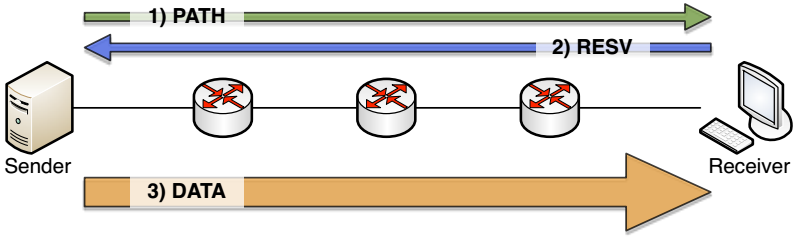
\includegraphics[scale = 0.4]{images/RSVP}
	\caption{Schema del protocollo RSVP.}
	\label{img:RSVP}
\end{figure}\\
Si consideri lo schema riportato in Figura \ref{img:RSVP}. Il protocollo RSVP si basa su due messaggi: \textit{PATH Message}, trasmesso dal \textit{Sender} verso i \textit{Receivers} (unicast o multicast) che indica il percorso che seguiranno i pacchetti, e \textit{RESV Message}, trasmesso dai \textit{Receivers} verso il \textit{Sender} in risposta al suo PATH, eventualmente modificando alcuni parametri. Vediamo più nel dettaglio come funzionano questi due tipi di messaggio. Nel messaggio PATH il Sender avvia una sessione RSVP, inserisce nel PATH message il \textit{Sender Template} (i.e. indirizzo IP e numero di porta) ed il \textit{Sender Tspec}, che descrive le caratteristiche del traffico dati che sarà generato; ciascun router memorizzerà il Sender Template, installerà lo stato della richiesta, e potrà aggiornare l'\textit{Adspec}, che riassume le caratteristiche di QoS del percorso fatto fino a quel router. Nel messaggio RESV, il Receiver riceve il PATH contenente anche una traccia del percorso fatto dal PATH e genera un RESV message, contenente il \textit{FilterSpec} (i.e., indirizzo IP e numero di porta del Receiver) ed il \textit{Flowspec} (descrive la QoS che il Receiver richiede); l'Admission Control di ogni router effettua l'ultimo controllo per determinare se le risorse sono disponibili ed in caso non lo siano viene generato un messaggio d'errore per il Receiver; infine ciascun router si aggiorna tramite il Filterspec e il Flowspec.\\
Per avere maggior controllo sulla QoS delle applicazioni, RSVP prevede diversi \textquotedblleft reservation styles", fra cui: \textit{Fixed-Filter (FF)}, in cui vi è una prenotazione di banda per ogni utente chiamante (es.: videoconferenza con requisiti di ritardo stringenti), e \textit{Shared-explicit (SE)}, in cui più utenti chiamanti nella stessa sessione possono dividere una prenotazione di risorse (es.: voiceconference dove solo uno per volta può parlare). RSVP supporta anche il multicast: riassume le prenotazioni provenienti da ciascun flusso, allocando sul nodo la maggior banda richiesta, e poi trasmette il Flowspec totale al router vicino (farà admission control sul flusso totale). È molto flessibile. Si noti che RSVP e IntServ sono \textit{unidirezionali}: per una \textquotedblleft telefonata" VoIP servono due sessioni IntServ.\\
Gli aspetti positivi sono: allocazione dinamica della banda, supporto quasi completo di RSVP, ed è un protocollo relativamente maturo, e dunque più stabile e diffuso. Vi sono però diversi problemi, per il quale non viene usato, tra cui: aggiornamento continuo (ogni 30 secondi) che comporta un notevole aumento del traffico di segnalazione, richiesta di memorizzazione di molti oggetti relativi ad ogni flusso su ogni router, necessita di una rete con buon Best Effort e routing stabile (le tabelle non devono variare troppo). In pratica \textit{non è scalabile in reti di elevate dimensioni}. Infine, basta un solo router che non supporta IntServ per farlo cadere.

Il DiffServ è il contrario del IntServ. Il modello DiffServ si basa sul multiplexing statistico, ossia si dividono (dinamicamente) le risorse di rete tra un numero limitato di diversi \textquotedblleft tipi" di traffico, in modo che ciascuno sia sostanzialmente isolato dagli altri. La complessità si sposta all'edge della rete, dove si classificano i singoli pacchetti, si marchiano (\textit{colorazione}) e si aggregano per poi inviarli nel core; flussi provenienti da diverse applicazioni vengono aggregati insieme e trattati allo stesso modo. Si opera in pratica su aggregati. Nel core il flusso aggregato riceve un trattamento relativo alla classe di servizio (al colore) dei pacchetti che contiene (\textit{Per-Class}, non più Per-Flow). Non vi è più segnalazione (RSVP), né admission control, e dunque è necessario ricorrere al \textit{provisioning} delle risorse a priori (vengono allocate più risorse del necessario), e viene controllato all'edge che il traffico immesso non sia eccessivo. Non vi è più traffico di segnalazione. La base del DiffServ e nel modo in cui si \textquotedblleft colorano" i pacchetti e come il \textquotedblleft colore" viene trattato. Il colore viene inserito nei bit di header IP del Traffic Class (IPv6) e nei bit di header IP del Type of Service (IPv4), precisamente nel \textit{DSCP} (6 bit). Abbiamo inoltre il \textit{Per-Hop-Behavior (PHB)}, che definisce il servizio che il pacchetto riceverà a ciascun hop nella rete, ed il \textit{Behavior Aggregate (BA)}, un  gruppo di pacchetti (aggregato) con stesso DSCP: nella rete si applica un PHB ad ogni BA.\\
I nodi DiffServ agiscono diversamente tra \textit{Edge} e \textit{Core}.
\begin{figure}[htbp]
	\centering
	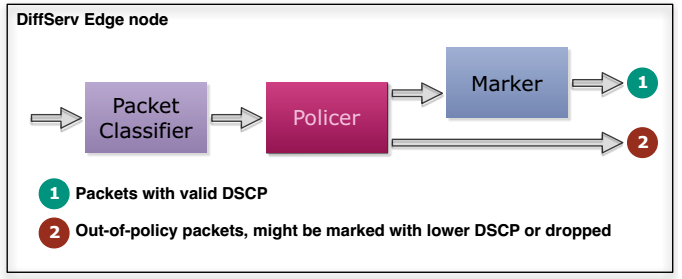
\includegraphics[scale = 0.4]{images/diffserv-edge-node}
	\caption{DiffServ Edge node.}
	\label{img:diffserv-edge-node}
\end{figure}
In Figura \ref{img:diffserv-edge-node} è riportato un nodo di bordo (edge) DiffServ. Il Packet Classifier implementa un metodo di classificazione, il Policer effettua un controllo del rispetto del Service Level Agreement ed il Marker provvede ad effettuare una marchiatura con il DSCP appropriato. Abbiamo visto che in un core node vi è un BA Classifier, basato sul DSCP e su altri parametri di livello MAC, da cui si ricava il PHB, e lo scheduler, basato sul PHB. Si tenga presente che il PHB ed il DSCP non sono la stessa cosa: il PHB indica la QoS da assegnare al pacchetto, il DSCP sono sei bit che indicano il colore del pacchetto. Un router ricava il PHB dal BA classifier. L'insieme dei PHB compongono il Behavior Aggregate (BA). Esistono tre tipi di PHB:
\begin{itemize}
	\item \textit{Default}. È il Best Effort tradizionale, non vi è QoS.
	\item \textit{Expedited Forwarding (EF)} -- RFC 2598. Connessioni con basse perdite, basso ritardo e basso jitter. Usa un solo DSCP (101110, 46) per immettere il pacchetto nella coda a più alta priorità nei router di rete (con WFQ ad esempio).
	\item \textit{Assured Forwarding (AF)} - RFC 2597. Definisce 4 classi di servizio relative, ciascuna con tre livelli di precedenza di scarto; usa 12 distinte combinazioni di DSCP. Il SLA dipende da: classe AF (risorse allocate), livello di traffico di quella classe, drop precedence (in caso di congestione).
\end{itemize}
Il PHB AF e quello maggiormente in uso, e definisce una matrice di $4\times 3$ possibili comportamenti (4 classi con 3 probabilità di scarto ciascuna):
\begin{table}[htbp]
	\centering
	\begin{tabular}{l|c|c|c|c|}
		& Class 1 & Class 2 & Class 3 & Class 4 \\
		\hline
		\begin{tabular}{l}Low\\Drop\end{tabular} & \begin{tabular}{c}001010\\$10_{10}$ $12_8$\end{tabular} & \begin{tabular}{c}010010\\$18_{10}$ $22_8$\end{tabular} & \begin{tabular}{c}011010\\$26_{10}$ $32_8$\end{tabular} & \begin{tabular}{c}100010\\$34_{10}$ $42_8$\end{tabular} \\
		\hline
		\begin{tabular}{l}Medium\\Drop\end{tabular} & \begin{tabular}{c}001100\\$12_{10}$ $14_8$\end{tabular} & \begin{tabular}{c}010100\\$20_{10}$ $24_8$\end{tabular} & \begin{tabular}{c}011100\\$28_{10}$ $34_8$\end{tabular} & \begin{tabular}{c}100100\\$36_{10}$ $44_8$\end{tabular} \\
		\hline
		\begin{tabular}{l}High\\Drop\end{tabular} & \begin{tabular}{c}001110\\$14_{10}$ $16_8$\end{tabular} & \begin{tabular}{c}010110\\$22_{10}$ $26_8$\end{tabular} & \begin{tabular}{c}011110\\$30_{10}$ $36_8$\end{tabular} & \begin{tabular}{c}100110\\$38_{10}$ $46_8$\end{tabular} \\
		\hline
	\end{tabular}
	%\caption{}
	%\label{tab:PHB-AF}
\end{table}\\
La classe è definita nei primi tre bit, mentre la drop precedence è definita nei secondi tre bit. Si noti che la classe non definisce una priorità relativa: è compito dell'ISP definire le associazioni di priorità, ossia i PHB ed i BA.\\
Vantaggi del DiffServ:
\begin{itemize}
	\item Maggiore scalabilità, la complessità viene spostata sull'edge.
	\item Non è più necessario il protocollo di segnalazione RSVP: minor overhead.
	\item Clienti diversi possono essere \textquotedblleft partizionati" in varie classi.
	\item Si integra piuttosto bene con le tecnologie di livello rete.
\end{itemize}
Svantaggi del DiffServ:
\begin{itemize}
	\item La diffusione dei DiffServ su domini di providers diversi impone accordi di peering bilaterali, difficili da gestire.
	\item Bisogna non immettere in rete traffico in eccesso, cosa piuttosto complicata. L'Admission Control manca, quindi bisogna usare il \textit{Traffic Engineering}\footnote{Con il termine Traffic Engineering si indicano tutte le tecniche online o offline di misurazione e previsione del traffico atte a prevedere una QoS ed implementare delle tecniche qualsiasi per ottimizzare l'uso della rete e delle risorse.}: si predice il traffico di un determinato BA e si tarano il
	routing, le precedenze, gli scheduler, etc. in modo da ottenere la QoS voluta.
	\item È QoS \textit{statistica}, quindi non funziona su reti con poca banda.
	\item Va comunque rispettata la regola di Van Jacobson: se vogliamo mantenere la QoS su una rete in cui non vi sono metodi di supporto alla QoS (over-provisioning), l'occupazione della rete deve essere $\approx 30\%$. I link non devono comunque superare il 50-70\% della loro capacità, in caso di sistema statistico.
\end{itemize}
DiffServ può funzionare bene, con occupazioni della rete anche superiori al 70\%, ma deve essere accoppiato con altri metodi di supporto alla QoS, come MPLS che si occupa della riservazione delle risorse.

\section{MPLS}
In un router convenzionale le funzioni di forwarding sono ad alto costo computazionale e costituiscono un collo di bottiglia in caso di link ad elevate capacità (terabit). \textbf{MPLS (Multiprotocol Label Switching)} semplifica le funzioni di forwarding attraverso l'uso di un approccio completamente diverso, introducendo un meccanismo orientato alla connessione all'interno del network IP. MPLS è una tecnica level 2 mutuata dall'approccio ATM.\\
Nella metà degli anni '90 gli switch IP erano molto più lenti degli switch ATM, poiché gli switch ATM operano sul forwarding del VCI/VPI. Vennero quindi proposte numerose soluzioni proprietarie per adottare tecniche di label forwarding all'IP, da Cisco Systems (Tag Switching), IBM (aggregate route-based IP switching) e Cascade (IP Navigator): tutte avevano in comune l'idea di adottare il label switching in maniera simile a quello usato da ATM. Dunque nel 1997 IETF aprì un gruppo di lavoro per definire MPLS come approccio standard. MPLS viene definito come standard nel 2001 (primo set di Proposed Standard), ma negli ultimi anni '90, però, erano già stati prodotti switch IP nativi veloci quanto quelli ATM (i.e., switch hardware-based a livello IP), dunque non era più necessario usare IP over ATM per fare il routing su reti ad altissima velocità. MPLS offre tuttora cose che l'IP switching non permette (bene): QoS support, Traffic Engineering, Virtual Private Networks (soprattutto in IPv4) e Multiprotocol Support.\\
Come abbiamo visto, DiffServ e IntServ hanno entrambi delle controindicazioni. In particolare, i network provider hanno necessità di: garantire specifici quantitativi di banda per determinate applicazioni, controllare la latenza/jitter, garantire i livelli di QoS specificati negli SLA e configurare la QoS in base agli utenti. MPLS fornisce un framework connection-oriented all'interno del quale è possibile soddisfare questi requisiti.\\
Il routing \textquotedblleft tradizionale" IP (e.g., OSPF) non prevede cammini multipli e opera su base pacchetto. MPLS opera su base \textit{flusso} permettendo di usare route multiple tra punti di ingresso/uscita dal network, ciascuna soggetta a QoS. Il re-routing in MPLS è esso stesso soggetto a QoS, ma è possibile  operare il cosiddetto traffic engineering nel senso di ottimizzazione delle risorse di rete in base alle richieste di ciascun flusso. Si noti che il flusso MPLS non corrisponde ai concetti di flusso DiffServ o IntServ.\\
MPLS fa il routing in maniera \textquotedblleft blind", quindi permette di ottenere: separazione dei flussi di una VPN da quelli del normale traffico e garantire ai flussi della VPN un elevato gradi di sicurezza. Inoltre MPLS non ha necessità di \textquotedblleft vedere" nemmeno l'header IP, per cui si possono creare VPN con crittografia anche degli header IP.\\
MPLS non si basa su alcuna tecnologia in particolare, è possibile avere switch IP MPLS, ATM MPLS e Frame Relay MPLS. Inoltre gli switch MPLS-enabled possono coesistere con switch non-MPLS, e MPLS può \textquotedblleft trasportare" qualsiasi tipo di protocollo, non soltanto IP: è quindi \textit{multiprotocollo}.\\
Un network MPLS consiste in un set di nodi MPLS contigui detti \textbf{LSR (Label Switching Routers)}. Una label definisce un flusso di pacchetti tra due endpoint o, nel caso di multicast, tra un ingress node e molti egress nodes. Un flusso con una label si chiama \textit{FEC (Forward Equivalence Class)} e per ciascuna FEC viene stabilito un path attraverso il network. Una FEC è caratterizzata anche dalla QoS richiesta per quella FEC. Si noti il mix tra concetti IntServ e DiffServ. Mentre per IntServ un flusso è unidirezionale tra un nodo ed un altro (end-to-end), per DiffServ è dato dai pacchetti che hanno lo stesso colore e per MPLS è dato dai pacchetti che hanno la stessa label.
\begin{figure}[htbp]
	\centering
	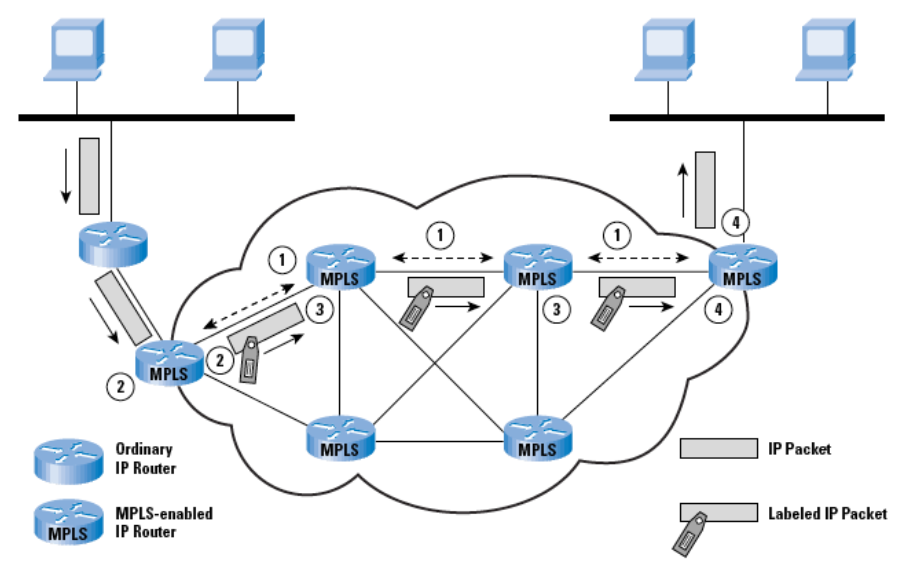
\includegraphics[scale = 0.4]{images/MPLS}
	\caption{Funzionamento MPLS.}
	\label{img:MPLS}
\end{figure}
È possibile in questo modo aggregare dei dati che hanno bisogno della stessa QoS. In Figura \ref{img:MPLS} è riportato il funzionamento del MPLS. Prima del routing/delivery dei pacchetti di una FEC si deve stabilire il path (\textit{LSP - Label Switched Path}). I parametri di QoS del FEC determinano la quantità di risorse assegnate a quel FEC e le politiche di accodamento e scarto per quel FEC. Per far ciò si fa ricorso sia ad algoritmi IGP (come OSPF) per costruire e mantenere la topologia della rete sia a politiche di assegnazione e distribuzione delle label. Le label sono locali tra due LSR e possono essere impostate manualmente o tramite protocolli come il Label Distribution Protocol (LDP) o l'RSVP-TE. Quindi una label potrebbe non essere uguale per tutto il percorso: ogni nodo può decidere se cambiarla o meno. La FEC invece rimane uguale. Abbiamo che:
\begin{enumerate}
	\item Un pacchetto entra nel ingress edge LSR, gli viene assegnata una label (FEC) in base a una serie di parametri simili a quelli DiffServ e gli viene attaccata una label (assgenazione ad un LSP) se esiste un LSP adeguato. Alternativamente l'edge LSR coopera con gli altri LSR per costruire una nuova LSP.
	\item All'interno del dominio MPLS un LSR si limita a: togliere la label in ingresso, aggiungere la label di uscita e fare il forwarding.
	\item L'egress LSR toglie la label e fa il forwarding \textquotedblleft tradizionale" sui nodi non-MPLS.
\end{enumerate}
MPLS prevede inoltre un una gestione centralizzata del permette di scegliere il path ottimo in modo globale.
\begin{figure}[htbp]
	\centering
	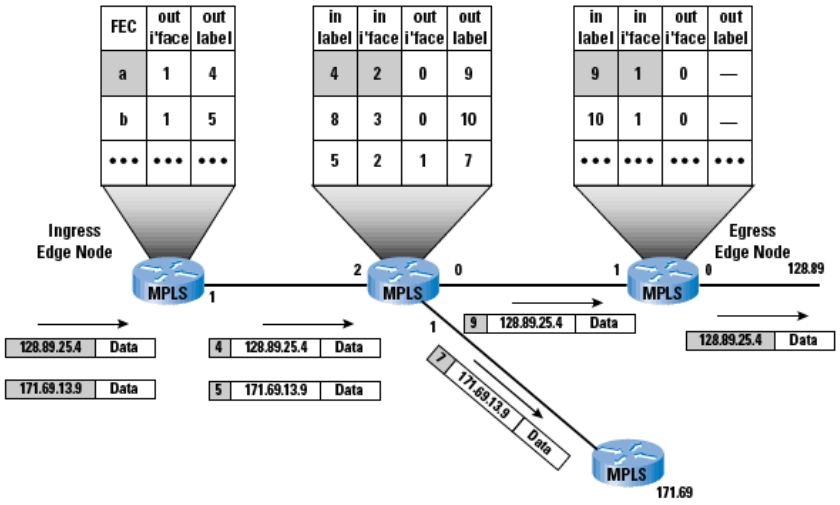
\includegraphics[scale = 0.4]{images/MPLS-example}
	\caption{Esempio di funzionamento MPLS.}
	\label{img:MPLS-example}
\end{figure}\\
In Figura \ref{img:MPLS-example} è riportato un esempio di funzionamento dell'MPLS. Entrano due pacchetti ed ad ognuno viene assegnata una FEC diversa (a, b) dal primo router; i nodi interni non guardano più la FEC, ma solo le label ed eventualmente le modificano.\\
Contrariamente ad ATM, che ha solo 2 livelli di stacking delle label (VCI e VPI), MPLS permette uno stacking virtualmente illimitato. Un LSR può assegnare una label a un gruppo di LSP in ingresso unendoli in un singolo LSP di uscita. All'uscita dal tunnel gli LSP vengono differenziati nuovamente. Questo è ottenuto \textit{aggiungendo} una label (stacking) alla label già presente. Le label vengono processate in ordine LIFO. Il numero di livelli di stacking non è definito, quindi non è limitato a due.
\begin{figure}[htbp]
	\centering
	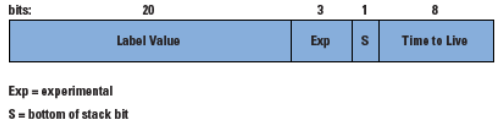
\includegraphics[scale = 0.55]{images/label-format}
	\caption{Formato di una label.}
	\label{img:label-format}
\end{figure}\\
In Figura \ref{img:label-format} è riportato il formato di una label. Il campo \textit{label value} (20 bits) indica la label con significato locale; il campo \textit{exp} (3 bits) contiene dati sperimentali, come campo DS o guide relative al PHB; il campo \textit{S} (1 bit) è posto a 1 se la label è l'ultima dello stack, 0 altrimenti; il campo \textit{TTL} (8 bit) rappresenta il Time To Live.
\begin{figure}[htbp]
	\centering
	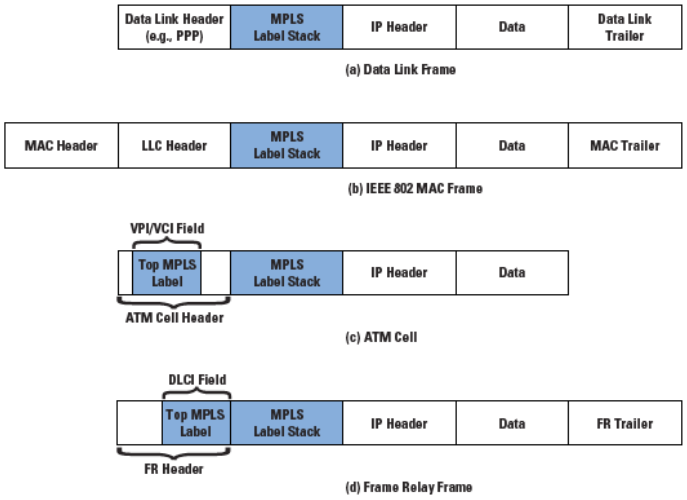
\includegraphics[scale = 0.45]{images/label-position}
	\caption{Posizione della label nei vari tipi di pacchetto.}
	\label{img:label-position}
\end{figure}\\
In Figura \ref{img:label-position} è riportata la posizione della label nei vari tipi di pacchetto: in generale questa viene sempre posta prima dell'header IP. Dal momento che l'MPLS \textit{non} esamina l'header IP, non può controllare o modificare il campo TTL dell'IP, quindi il TTL IP (o equivalente) viene replicato nella label. All'egress LSR il campo TTL della label viene ricopiato nel campo TTL dell'header IP (o equivalente); per IPv6 si usa il campo \textit{Hop Limit}. Si noti che solamente il TTL della label più \textquotedblleft esterna" ha significato. Se la label viene rimossa (i.e., fine di un tunnel) si ricopia il valore nella label più esterna corrente.\\
Per poter funzionare efficacemente è necessario poter stabilire l'LSP a cui assegnare una determinata FEC (o crearlo). MPLS permette due opzioni:
\begin{enumerate}
	\item \textbf{Hop-by-hop routing}. Ciascun LSR sceglie autonomamente il prossimo LSR. Funzionalmente equivalente all'uso di OSPF, si appoggia ai protocolli IGP. Permette i vantaggi dell'uso delle label ma \textit{non} quelli del traffic engineering, QoS, etc.
	\item \textbf{Explicit routing}. Con l'explicit routing l'ingress o l'egress LSR determinano il path completo (o quasi) del routing. L'explicit routing può essere \textit{strict} o \textit{loose}. Nello \textit{strict explicit routing} l'LSP è definito completamente tramite gli LSR coinvolti. Nel \textit{loose explicit routing} l'LSP è definito tramite alcuni degli LSR coinvolti, lasciando un margine di incertezza sugli LSR non specificati. Serve per i link di backup o laddove vi siano topologie mesh equivalenti. L'explicit routing può essere statico (LSP definiti a priori) o dinamico.
\end{enumerate}
Per l'explicit routing dinamico serve che il protocollo IGP sottostante dia metriche ricche sullo stato della rete. OSPF non è per esempio sufficiente. Sono stati definite estensioni all'OSPF per questo. La route è calcolata in base agli attributi dei link tra gli LSR (banda, ritardi, PER, PLR, etc.) ed agli attributi della FEC (QoS richiesta). Gli algoritmi di calcolo della route che si basano sugli attributi sono detti \textit{constrain-based routing algorithms} e sono notevolmente più complessi degli algoritmi tradizionali, ma vengono eseguiti solo alla creazione del'LSP.\\
Per far si che le label siano correttamente assegnate (sono locali) si devono impiegare dei protocolli di distribuzione delle label; ne esistono svariati, ad esempio LDP, RSVP-TE, etc. Il protocollo di distribuzione delle label è comunque legato al tipo di LSP (esplicito, dinamico, strict, loose) e al tipo di protocollo di routing implementato. La tecnica più usata è quella backward, che partendo dall'egress LSR informa ogni LSR precedente della label locale assegnata; non è tuttavia così semplice, dal momento che un LSP può contenere traffico multicast -e- many-to-one (il contrario del multicast).\\
Esiste una generalizzazione dell'MPLS, il \textit{GMPLS (Generalized MPLS)}. Lo scopo di GMPLS è quello di estendere i concetti di management propri di MPLS a reti di natura diversa e di estendere l'introperabilità. È un set di protocolli di management degli LSP e di setup degli LSP sui diversi tipi di rete. In particolare il focus è sul setup degli LSP, sul mantenimento della QoS e sul miglioramento della fault-tolerance della rete. È tuttavia ancora un work-in-progress, mentre l'adozione di MPLS è un dato di fatto: l'evoluzione e l'uso su larga scala di GMPLS è tuttora un'incognita. Alla fine dei conti non interessa molto, in generale, l'evoluzione di GMPLS perché al momento non vi sono forti necessità pratiche e concrete da parte degli ISP.

\section{Network Management}
Si consideri il diagramma riportato in Figura \ref{img:management-elements} che rappresenta gli elementi del management e come questi di interfacciano tra loro.
\begin{figure}[htbp]
	\centering
	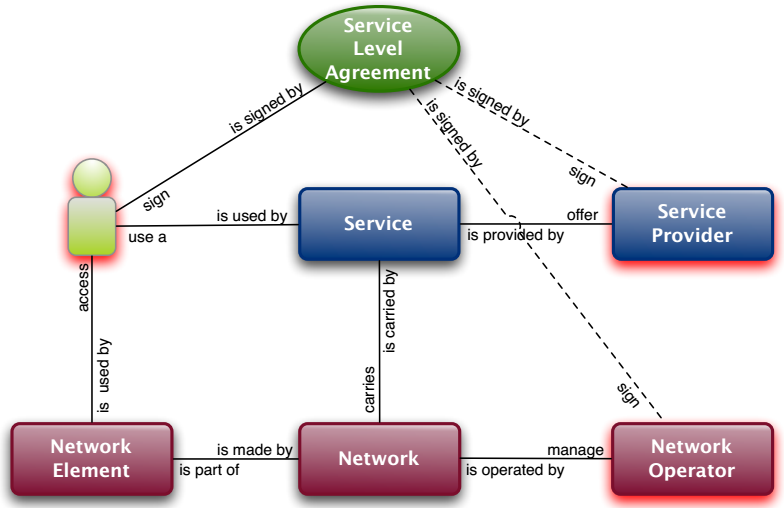
\includegraphics[scale = 0.55]{images/management-elements}
	\caption{Elementi del management.}
	\label{img:management-elements}
\end{figure}
L'utente usa un servizio che è gestito da un Service Provider. Il servizio e fornito tramite il Network, gestito dal Network Operator. Gli SLA regolano i rapporti tra Utente, Service Provider e Network Operator. Supposto che il Network Operator sia \textquotedblleft consapevole" dei servizi che vengono veicolati, il suo obiettivo è quello di gestire la rete, in accordo con lo SLA, tra lui e il Service Provider. Se il Network Operator non e interessato ai servizi, allora lo SLA di riferimento è quello tra lui e l'Utente.
\begin{figure}[htbp]
	\centering
	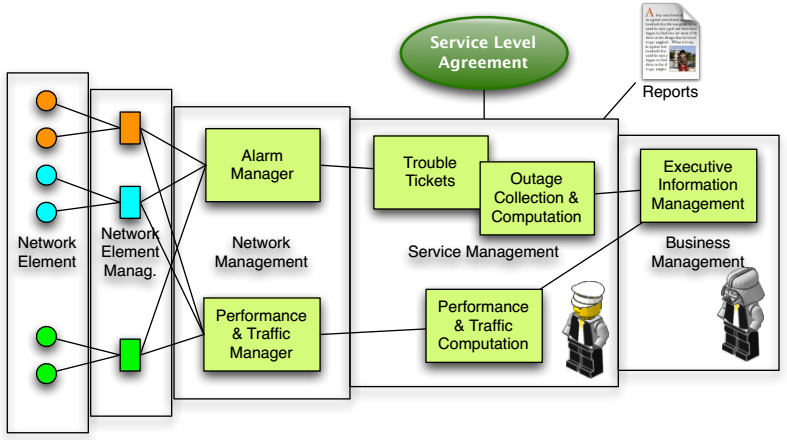
\includegraphics[scale = 0.55]{images/management-elements-1}
	\caption{Elementi del management.}
	\label{img:management-elements-1}
\end{figure}\\
Si consideri adesso la Figura \ref{img:management-elements-1}. I colori nel primo strato sono in base al vendor. Gli elementi di rete vengono gestiti attraverso due layer di management (uno tecnico ed uno funzionale). Il livello funzionale a sua volta è \textquotedblleft guidato" da un livello di service management, che è diretto dal rispetto degli SLA. Il tutto è sottomesso ai livelli di Business Management. L'ultimo strato (quello più a destra) è l'unico ad essere realizzato da esseri umani. Gli allarmi finiscono nei Trouble Tickets che rappresentano il modo in cui, all'interno del Network Management, viene gestito un evento all'interno della rete (anche eventi esterni). I Trouble Tickets finiscono negli Outage Collection \& Computation, che effettuano delle statistiche sui guasti, e nel Performance \& Traffic Computation, che effettuano delle statistiche sugli stati della rete. Ciò che è gestito da ognuno di queste componenti è definito nel SLA. Il management si differenzia in base alle tipologie di rete: vediamole. Il Service Management si occupa della gestione dei Servizi e dei Servers che li operano. Si svolge (quasi) tutto a livello applicativo. Con Backbone Network Management si intendono reti di grandi dimensioni, apparati e links ad altissima velocità (molti clienti). Le Access Network Management sono reti di piccole dimensioni, apparati a bassa velocità; vi è un contatto diretto con gli utenti. Le LAN Network Management sono reti di piccole dimensioni. Vi è un contatto diretto con gli utenti ed una gestione congiunta dei servizi.

È molto importante definire i domini di competenza. È abbastanza chiaro che nella fruizione di un servizio i dati dell'utente attraversano un numero spesso consistente di aree sotto il controllo (management) di diverse entità. Le diverse entità devono essere in contatto tra di loro al fine di mantenere il servizio attivo, altrimenti si rischia di avere un \textquotedblleft rimpallo di competenze". Si ponga attenzione infine al fatto che l'utente stesso è un dominio di competenza, nel senso che gli apparati utente sono spesso gestiti dall'utente stesso. Se si deve offrire un servizio garantito questo elemento di incertezza è estremamente importante (esempi: il jailbreak dell'iPhone, ma anche l'aggiornamento del firmware dei telefoni aziendali).\\
Per gestire un sistema (una rete o qualsiasi altra cosa) occorre avere un metodo e degli strumenti. Entrambi sono indispensabili e paritetiche. Considerarne solo una porta semplicemente al fallimento. In letteratura si trovano due \textquotedblleft approcci", che in realtà non sono diversi, ma complementari: ISO/OSI, centrato sul metodo, e IETF, centrato sui protocolli; è una falsa dicotomia, in quanto l'uno sfrutta elementi dell'altro.

ISO/OSI definisce 5 \textbf{aree funzionali}, e divide i compiti del Network Management tra di esse. Le aree rappresentano un modello di organizzazione del lavoro ed assolvono al compito di creare un sistema funzionale ed efficace per gestire il Network. ISO/OSI definisce anche un protocollo: il CMIP (e il CMIS), ma non si usano perché troppo complessi. Un punto di forza del CMIP/CMIS è però la \textit{gestione distribuita}, che manca nel modello IETF. Le aree funzionali ISO/OSI sono (F-CAPS to remember):
\begin{enumerate}
	\item \textbf{Fault}. Gestione dei guasti e degli allarmi. Comprende: il riconoscimenti tempestivo dei guasti sulla rete (apparati di rete, server, connessioni), log dei guasti e degli allarmi, procedure aziendali dedicate, test diagnostici, il rispetto delle specifiche di contratto sul ripristino dei servizi, gestione del call center dedicato agli allarmi e dei guasti, interfacciarsi con il cliente, allarmi dovuti a guasti effettivi o a superamento di soglie prestazionali.
	\item \textbf{Configuration}. Gestione delle configurazioni. I principali compiti sono: la raccolta e distribuzione di dati sullo stato delle risorse di rete, l'inizializzazione e modifica delle configurazioni degli apparati, modifiche on-line o off-line della configurazione, variazione della configurazione per l'ottimizzazione delle prestazioni, configurazione di router, firewall, switch, provisioning delle connessioni fisiche.
	\item \textbf{Accounting}. Gestione degli account e dei costi dei servizi. I principali compiti sono: la determinazione/modifica  dei diritti e caratteristiche di accesso al servizio in base al contratto stipulato, il billing dei servizi (addebitamento dei costi agli utenti finali), la definizione di limiti di utilizzo delle risorse da parte degli utenti, il calcolo di costi combinati per l'impiego di più risorse nell'ambito di un servizio (e.g. problema del roaming in reti cellulari e nelle reti wireless LAN di nuova generazione per l'accesso a Internet per utenti mobili).
	\item \textbf{Performance}. Gestione e miglioramento delle prestazioni. Comprende: il monitoraggio delle prestazioni della rete in base alle specifiche contenute nel Service Level Agreement con il cliente, i log delle prestazioni monitorate e report agli utenti finali, la modifica dell'allocazione delle risorse della rete per soddisfare le richieste dei clienti, l'adozione di misure preventive per evitare situazioni di congestione o di disservizio.
	\item \textbf{Security}. Gestione della sicurezza e degli accessi. I principali compiti sono: l'analisi delle aree di rete a rischio (es. database con informazioni sensibili sui clienti), l'adozione di piani per la sicurezza aziendale sia fisica che di rete, il controllo ed il logging degli accessi (passwords, diritti di accesso), test di vulnerabilità sulla rete e sugli ambienti fisici di accesso a server e database.
\end{enumerate}
I principi di base sono il \textit{Separation of Concerns} (non duplicare le funzionalità) e l'\textit{Information Hiding} (non esporre l'implementazione, ma solo un servizio). Tra le diverse aree ISO/OSI devono esserci dei SAP (o equivalenti), ovvero semantiche e sintassi da rispettare; una di queste è rappresentata dai Trouble Ticket. Un \textit{Trouble Ticket} è un sistema (qualsiasi) che tiene traccia dei problemi, del loro stato, delle azioni per risolverli e delle deleghe relative al soggetto che ha in carico il problema stesso. È molto importante tenere presente che le aree ISO/OSI \textit{non sono layer di comunicazione} e non si programmano: servono per far lavorare gruppi di persone. Come protocollo si utilizza invece \text{SNMP} (Simple Network Management Protocol), che rappresenta uno dei possibili modi con cui gestire la rete e serve ad interrogare un elemento della rete da un server (il Network Manager).
\begin{figure}[htbp]
	\centering
	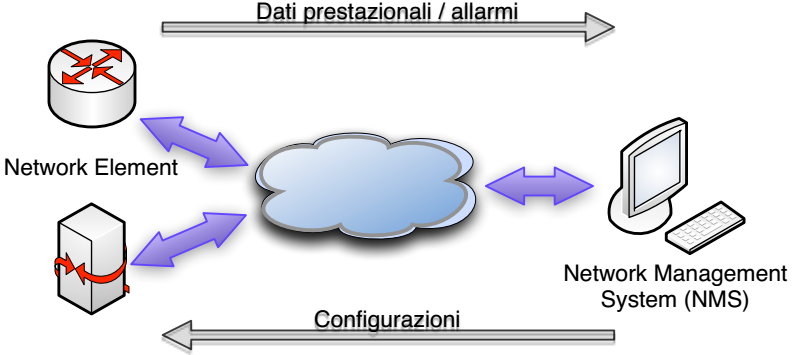
\includegraphics[scale = 0.55]{images/SNMP}
	\caption{Organizzazione di SNMP.}
	\label{img:SNMP}
\end{figure}\\
In Figura \ref{img:SNMP} è rappresentato il funzionamento di SNMP. In pratica, si opera direttamente sugli elementi \textit{attivi} ed indirettamente sugli elementi \textit{passivi}. La piattaforma di gestione (NMS) raccoglie i dati e agisce sui Network Elements (anche indirettamente). I principali elementi di un sistema di gestione di rete sono: il Network Element da gestire, il Network Management System (stazione di gestione), ed un protocollo di gestione. Nelle WAN i Network Elements sono: nodo Frame Relay o ATM, commutatore SDH, sistema optoelettronico per comunicazioni in fibra ottica, router IP di dorsale, collegamento punto-punto in fibra, etc. In una LAN, invece: server di mail, Web, FTP, stampanti, switch, Access Point per WLAN, database, pc uffici, centraline telefoniche/VoIP, etc. Servirebbe però un livello di \textit{astrazione} per uniformare in qualche modo gli elementi della rete. Dunque, il colloquio tra NMS e Network Element si svolge tra un processo \textquotedblleft Agent" sul Network Element ed un processo \textquotedblleft Manager" sul NMS, come illustrato in Figura \ref{img:SNMP-abstraction}.
\begin{figure}[htbp]
	\centering
	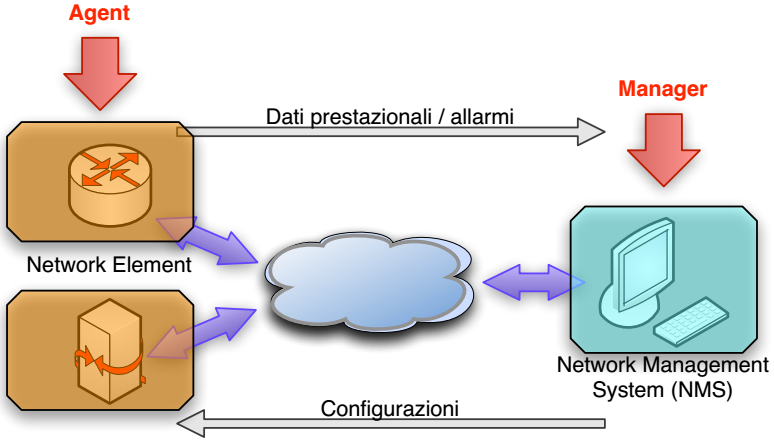
\includegraphics[scale = 0.55]{images/SNMP-abstraction}
	\caption{Paradigma Manager/Agent.}
	\label{img:SNMP-abstraction}
\end{figure}
Manager ed Agent colloquiano usando un protocollo di gestione (e.g. SNMP). Manager ed Agent sono due processi software che implementano \textit{oggetti logici}. Ciascun Network Element non è visto come un oggetto reale, ma come una rappresentazione logica di funzionalità, ossia un'astrazione. Questo permette di gestire diversi elementi \textquotedblleft diversi", ma che assolvono alle stesse funzioni (e.g. un wireless access point e un terabit router). Vi sono quindi due importanti parti: il \textit{protocollo di comunicazione} ed il \textit{sistema di rappresentazione logica}.\\
Il \textit{Management Information Base (MIB)} è il sistema attraverso cui si ha la rappresentazione logica degli oggetti gestiti nel database, organizzato come una \textquotedblleft directory" con struttura ad albero. Le variabili del MIB rappresentano gli attributi degli oggetti, che ne determinano lo stato, come ad esempio il massimo bit-rate di un'interfaccia, il numero di pacchetti in coda, etc. Sia il NMS che l'Agent condividono la conoscenza del MIB. Si noti che il MIB non è un database, ma un Information Base. La \textquotedblleft conoscenza" è relativa alla struttura e non al contenuto. In Figura \ref{img:SNMP-complete} è riportato lo schema completo del paradigma Manager/Agent.
\begin{figure}[htbp]
	\centering
	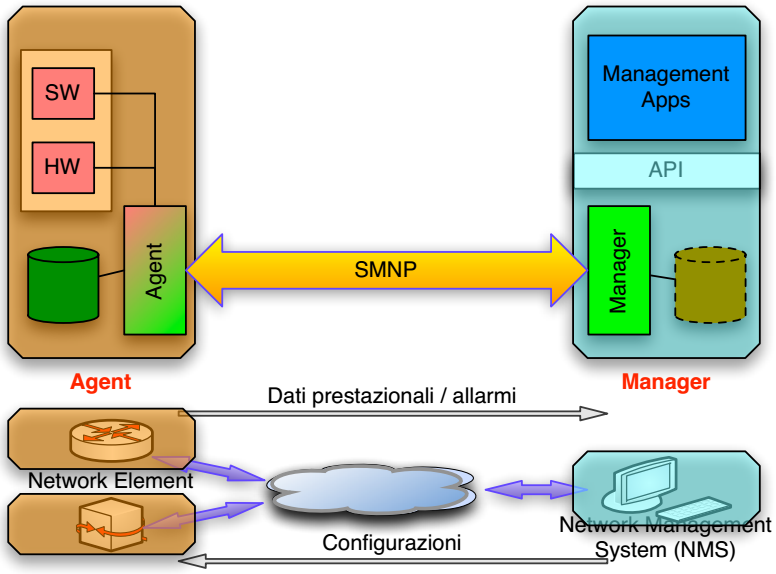
\includegraphics[scale = 0.45]{images/SNMP-complete}
	\caption{Paradigma Manager/Agent.}
	\label{img:SNMP-complete}
\end{figure}\\
Quindi, sostanzialmente, il MIB ha un'organizzazione ad albero, è contenuto nel processo Agent e contiene le variabili relative al Network Element gestito. Il Manager conosce la struttura ad albero del MIB, e la \textquotedblleft naviga" mediante i messaggi SNMP di request; il MIB deriva da una struttura logica ad albero più generale, l'albero delle registrazioni ISO.
\begin{figure}[htbp]
	\centering
	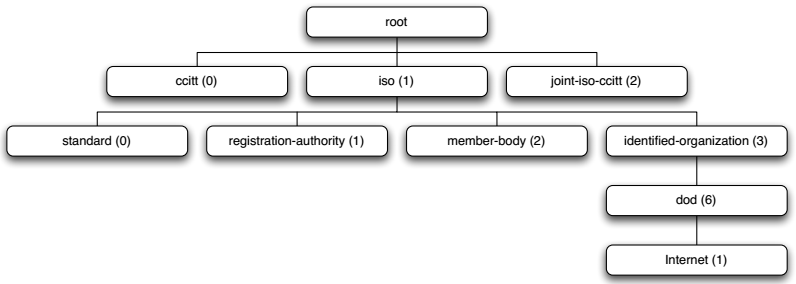
\includegraphics[scale = 0.55]{images/MIB-example}
	\caption{Esempio di Management Information Base.}
	\label{img:MIB-example}
\end{figure}\\
Si consideri l'esempio di MIB riportato in Figura \ref{img:MIB-example}. Chiamiamo con il termine \textit{registration tree} una directory di standard. Un elemento è identificato dal suo \textit{Object Identifier (OID)}, ossia la sequenza dei rami per raggiungerlo partendo dalla radice. Ad esempio, Internet OID $:= \{$iso org(3) dod(6) 1$\}$, oppure 1.3.6.1 (in formato numerico), oppure iso.org.dod.1 (in formato simbolico). I MIB SNMP sono estensioni dell'albero delle registrazioni. Il \textquotedblleft MIB name" è l'OID che indica la radice del sotto-albero che contiene il MIB. Ad esempio, \texttt{iso.org.dod.internet.management.mib-2} (1.3.6.1.2.1) è l'identificatore del MIB standard definito per gestire apparati TCP/IP. Sostanzialmente i dati del MIB sono memorizzati nelle foglie dell'albero ed i nodi interni del MIB rappresentano raggruppamenti logici di oggetti. Le entità multi-istanza vengono memorizzate sotto forma di tabelle. Dunque abbiamo delle \textit{variabili scalari}, che hanno un solo valore possibile, e delle \textit{tabelle}, che descrivono oggetti presenti in più istanze, come interfacce, connessioni, etc. Ogni colonna contiene tutti i valori di un attributo per le diverse istanze.
\begin{figure}[htbp]
	\centering
	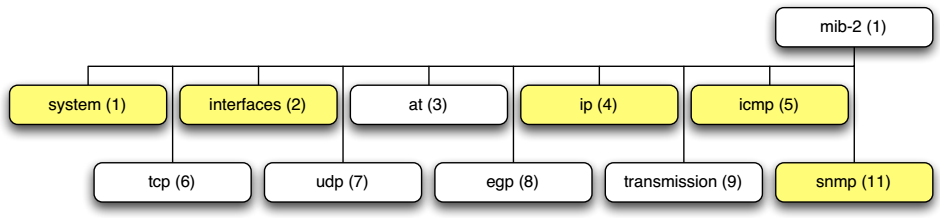
\includegraphics[scale = 0.55]{images/mib-2}
	\caption{Gerarchia di \texttt{mib-2}.}
	\label{img:mib-2}
\end{figure}\\
\texttt{mib-2} (RFC 1213) si occupa della gestione di apparati IP. Inizialmente furono definiti 10 gruppi per 171 \textquotedblleft classi" di oggetti gestiti. Come è possibile notare dalla Figura \ref{img:mib-2} i gruppi obbligatori sono: system, interfaces, IP, ICMP, SNMP. L'implementazione dei gruppi rimanenti è legata al tipo di dispositivo.\\
Il gruppo \texttt{system} (1.3.6.1.2.1.1) contiene le informazioni principali che fanno riferimento all'intero sistema: sysDescr (1), sysObjectID (2), sysUpTime (3), sysContact (4), sysName (5), sysLocation (6), sysServices (7). Il gruppo \texttt{interfaces} (1.3.6.1.2.1.2) contiene le informazioni principali sulle interfacce: ifNumber (1), ifTable (2) e tutte le opzioni e le operazioni relative alle entry di una tabella. Il gruppo \texttt{ip} contiene le informazioni principali sul livello IP.
\begin{figure}[htbp]
	\centering
	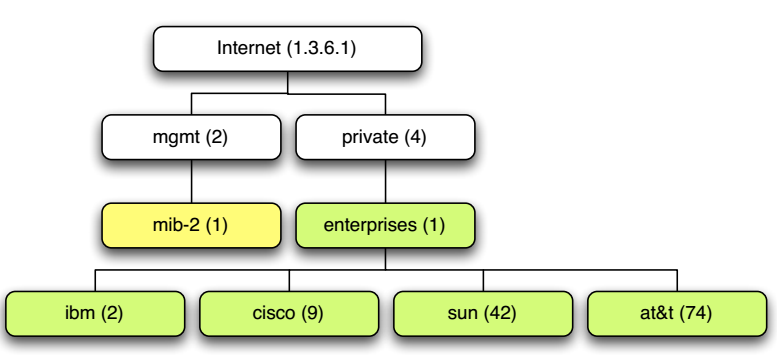
\includegraphics[scale = 0.55]{images/mib-extensions}
	\caption{Estensione di MIB.}
	\label{img:mib-extensions}
\end{figure}\\
Il MIB non è chiuso: molti pensano erroneamente che sia difficile da estendere. Infatti, come riportato in Figura \ref{img:mib-extensions}, il MIB si può estendere sotto 1.3.6.1.4.1.xx (ibm, cisco, sun, at\%t, etc.). Inoltre, se il MIB vuole rappresentare come identificare gli oggetti logici, l'SNMP è il protocollo con il quale il Manager e l'Agent comunicano e lavora su UDP. Le primitive SNMP (v2c e v3) sono molto semplici; queste si distinguono nelle primitive \textit{Manager to Agent}
\begin{itemize}
	\item GetRequest (reply: Response)
	\item GetNextRequest (reply: Response)
	\item GetBulkRequest (reply: Response * n)
	\item SetRequest (reply: Response)
\end{itemize}
e \textit{Agent to Manager}
\begin{itemize}
	\item SNMPv2-Trap
	\item InformRequest (reply: Response)
\end{itemize}
Vediamo adesso le versioni di SNMP.
\begin{itemize}
	\item \textbf{SNMPv1}. È incompatibile con le versioni successive e mancano \textit{GetBulkRequest} e \textit{InformRequest} (molto lento). Da evitare.
	\item \textbf{SNMPv2c}. È compatibile con SNMPv3, ma l'autenticazione è debolissima e la privacy è assente. L'autenticazione viene effettuata tramite la conoscenza di una \textit{community}; la community è trasmessa in chiaro ed identifica i permessi \textit{read} e \textit{write}. Da usare solo per \textit{get} (lettura), mai per \textit{set} (scrittura).
	\item \textbf{SNMPv3}. È usabile e \textquotedblleft sicuro" ed è molto più complicato rispetto all'autenticazione ed alla privacy. Dalla documentazione CISCO:
	\begin{itemize}
		\item Ogni utente appartiene ad un gruppo.
		\item Un gruppo definisce le politiche di accesso per un insieme di utenti. Una politica di accesso identifica ciò che gli oggetti SNMP rendono accessibile per lettura, scrittura o creazione.
		\item Un gruppo determina una lista di notifiche che i suoi utenti possono ricevere.
		\item Un gruppo definisce inoltre il modello ed il livello di sicurezza per i suoi utenti.
	\end{itemize}
\end{itemize}
Si consideri la Figura \ref{img:SNMP-role}. SNMP permette la comunicazione, ma le Management Apps comunicano End-to-End. Diventa dunque importante l'API tra SNMP Manager e le applicazioni tra l'Agent e la strumentazione.
\begin{figure}[htbp]
	\centering
	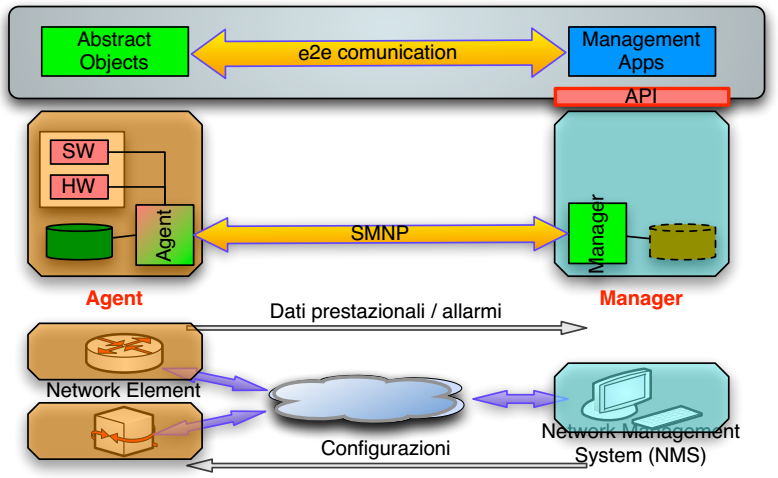
\includegraphics[scale = 0.55]{images/SNMP-role}
	\caption{Ruolo di SNMP.}
	\label{img:SNMP-role}
\end{figure}\\
Non sempre si hanno apparati che rispondono a SNMP: potremmo avere che il NMS si trova in una condizione in cui vi è un'interfaccia con una rete SNMP ed un'interfaccia con un'altra rete (e.g. ATM). La soluzione è quella di fare un proxy o delle traslazioni di protocollo.
\begin{figure}[htbp]
	\centering
	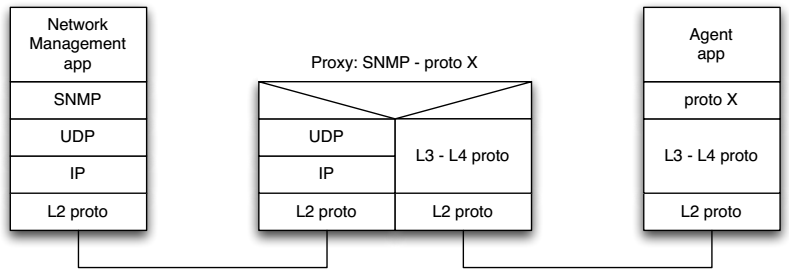
\includegraphics[scale = 0.55]{images/multiprotocol}
	\caption{Conversione da SNMP a protocollo X.}
	\label{img:multiprotocol}
\end{figure}\\
In Figura \ref{img:multiprotocol} è rappresentata la traslazione da un protocollo qualsiasi a SNMP. Se il protocollo X è di tipo Request/Response, allora serve un proxy; se il protocollo non è di tipo Request/Response, allora serve un gateway. I Proxy costano moltissimo, ma risolvono il problema dell'avere Manager differenti.
\begin{figure}[htbp]
	\centering
	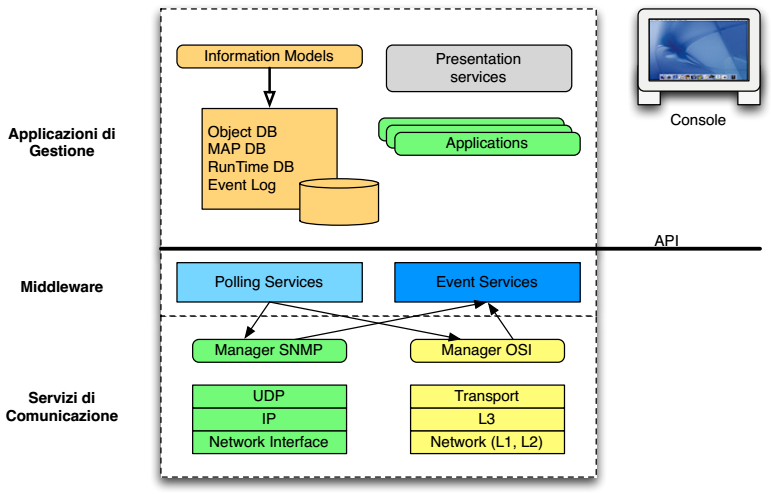
\includegraphics[scale = 0.55]{images/Ideal-Network-Management-System}
	\caption{Network Management System ideale.}
	\label{img:Ideal-Network-Management-System}
\end{figure}\\
In Figura \ref{img:Ideal-Network-Management-System} è riportato un Network Management System ideale. Ai livelli più bassi abbiamo i Servizi di Comunicazione: gli strati fisici e quelli di trasporto; nella parte sinistra abbiamo quelli SNMP, nella parte destra quelli del protocollo X col quale vogliamo interfacciarci. Gli strati fisici e quelli di trasporto possono essere benissimo diversi. Sopra ancora abbiamo i Manager SNMP ed un altro Manager qualsiasi. Questi servizi obbediranno a due macro-aree: Eventi in Polling (updates, interrogazioni periodiche) e gli Eventi di Allarme (eventi unsolicited). Questi due oggetti comunicano, tramite delle API, con un Information Model (simile al MIB, ma molto più esteso -- e.g. notifica un router guasto), dei Servizi di Presentazione (e.g. plot di grafici) e delle Applicazioni che automatizzano il tutto. Una Network Management Platform dovrebbe separare il livello di Comunicazione (SNMP o altro) da quello di Applicazione (automatica, console, etc.).

L'SNMP ha alcune limitazioni: i dati sono relativi ad un \textit{istante} ben preciso e l'overhead limita la risoluzione temporale del sampling (polling period). Per ovviare a questo problema si ricorre ad un altro sistema: \textbf{RMON (Remote MONitoring)}, che permette di collezionare, processare e fornire dati storici. RMON effettua l'analisi dei primi due livelli della pila OSI ed RMON 2 (RFC 2021), usato attualmente, è un'ulteriore estensione che effettua:
\begin{itemize}
	\item Un'analisi dei livelli più alti (fino al livello applicativo).
	\item Il miglioramento delle capacità di filtraggio dei pacchetti.
	\item Il miglioramento delle funzionalità in ambiente Multi-Manager.
	\item Il miglioramento delle capacità di elaborazione locale dei dati sull'agente.
\end{itemize}
RMON si \textquotedblleft interroga" tramite un MIB particolare con SNMP. Altri tools per l'analisi di reti sono: PING, Traceroute, mtr (traceroute + ping), ICMP, IPFIX, etc. \textit{IPFIX (Internet Protocol Flow Information eXport)} (RFC 5101) è un protocollo \textit{push} che deriva da NetFlow v9 (Cisco). In pratica la \textit{probe} analizza il traffico ed invia i dati ad un Collector tramite IPFIX. Dall'RFC: \textquotedblleft \textit{IPFIX considers a flow to be any number of packets observed in a specific timeslot and sharing a number of properties}". Altri strumenti, Network Management Systems, che permettono di fare Network Management sono:
\begin{itemize}
	\item \textbf{Nagios}. \textquotedblleft \textit{Nagios is a powerful monitoring system that enables organizations to identify and resolve IT infrastructure problems before they affect critical business processes.}"
	\item \textbf{OpenNMS}. \textquotedblleft \textit{OpenNMS is the world's first enterprise grade network management application platform developed under the open source model.}"
	\item \textbf{Cacti}. \textquotedblleft \textit{Cacti is a complete network graphing solution designed to harness the power of RRDTool's data storage and graphing functionality.}"
	\item \textbf{Zenoss}. \textquotedblleft \textit{Zenoss assures IT service delivery to applications, business services and real-time physical, virtual, and cloud-based infrastructures.}"
\end{itemize}
È importante controllare sempre che: sia supportato l'uso di Trouble Tickets, sia possibile definire utenti con privilegi diversi (Aree ISO/OSI) e che non sia un tool \textquotedblleft over-engineered" (cerca di far tutto, facendolo male). È comunque molto importante utilizzare sempre il terminale.

L'aspetto più complicato nel Network Management è il fattore umano: è difficile insegnare a lavorare alle persone, soprattutto sotto stress; è importante avere un metodo con cui affrontare le cose (considerazione personale del Prof. Pecorella).